\documentclass[11pt]{article}
\usepackage[a4paper,margin=25mm]{geometry}
\usepackage{amsmath,amssymb,amsthm,mathtools,mathrsfs,graphicx}
\usepackage[hypertexnames=false]{hyperref}
\newcommand{\C}{\mathbb C}\newcommand{\R}{\mathbb R}
\newcommand{\Tr}{\operatorname{Tr}}\newcommand{\diag}{\operatorname{diag}}
\newcommand{\rank}{\operatorname{rank}}\newcommand{\Rea}{\operatorname{Re}}
\newcommand{\Ima}{\operatorname{Im}}\newcommand{\dd}{\,d}
\newcommand{\eps}{\varepsilon}
\title{Original observations, mixed tensor sources, and arithmetic metric returns}
\author{Split-Zero research programme}
\date{20 September 2026; result SZ-20260920-055}
\newcommand{\im}{\operatorname{im}}
\newcommand{\Var}{\operatorname{Var}}
\newcommand{\Spec}{\operatorname{Spec}}
\newtheorem{theorem}{Theorem}
\newtheorem{lemma}[theorem]{Lemma}
\newtheorem{proposition}[theorem]{Proposition}
\begin{document}\maketitle
\begin{abstract}
The outgoing correction remains rank one after the actual observation,
but its square need not vanish. We compute its exact positive determinant
using the full original root polynomial, the compressed resolvent on the
original kernel, and a two-vector Gram determinant. Adjacent attained
metrics give an exact formula for the surviving correction. The established
conductor bounds then give its exponential degree profile, a nonlinear
heat limit, and the common-time four-cutoff value two. A separate bounded
two-scale logarithm has a strictly negative four-cutoff limit. Each claim
retains its own operator, metric, scale and original domain. The complete
conductor complement is carried through the same native current.
For general tensor families we calculate the collision exponents and
propagate the complete added-source covariance through the original
observation and kernel. An evaluated Gamma tensor-to-sum projection
then supplies explicit reference matrices for the arithmetic comparison.
\end{abstract}

The finite determinant calculation OD1--10 is derived here. The incoming
observed-heat continuation \cite{OHinput} supplies the nonlinear and
common-time calculation, proved below using the existing complete-window
conductor estimates FW46--52 \cite{FW}%
% BEGIN VERIFIED PUBLIC PROOF LINK
~\href{https://github.com/KokunoYumeto/zeta-function-research-reader/blob/5992ad50c0f2a06921f1fcaded7b4e38097c0739/workbenches/splitzero-tandem/continuations/20260920-original-kernel-mixed-determinants/providers/FULL_WINDOW_SOURCE_PRODUCTS.tex\#L28}{[proof FW1]}%
% END VERIFIED PUBLIC PROOF LINK
{}. The incoming logarithmic
continuation \cite{BLinput} supplies BL1--8. Its full-companion inverse
growth also overlaps the already completed SD19--25 \cite{SD}%
% BEGIN VERIFIED PUBLIC PROOF LINK
~\href{https://github.com/KokunoYumeto/zeta-function-research-reader/blob/5992ad50c0f2a06921f1fcaded7b4e38097c0739/workbenches/splitzero-tandem/continuations/20260920-original-kernel-mixed-determinants/providers/ORIGINAL_SPECTRAL_DETERMINANT.tex\#L34}{[proof SD1]}%
% END VERIFIED PUBLIC PROOF LINK
{}; it is
not counted again. No existence of an off-critical zero is asserted.

\section{The actual source, quotient and boundary}
Fix an actual hypothetical quartet of zeros of the original source,
$\rho=1/2+\delta+i\gamma$, $0<\delta<1/2$, $\gamma>2$, with
fixed multiplicity $m_0$. Retain $k\equiv1\pmod4$, $e=1+k(m_0-1)$,
$q=e(k+1)^2$, $c=k/2$ and
\begin{equation}\tag{OD1}
 Q(y)=\prod_{a,b=0}^{k}
 [y-(2b-k)\gamma+i(2a-k)\delta]^e,
 \quad E=\C[y]/(Q),\quad M[P]=[yP].
\end{equation}
The physical coordinate is $S=c+iy$. The original source measure is
$dm_k=w_h^{*k}(y)\dd y$, where
$w_h(y)=|(2\xi/h)(1/2+iy)|^2/(2\pi)$. For each original cutoff
$q-1\le N\le2q$, $G=G_N$ is the attained minimum of this entire
source over the entire ideal $(Q)$. Let $C=C_N$ be compression of
physical multiplication by $y$ to that attained source space.
It is selfadjoint for $G$. With the original $S$-monic orthogonal
polynomials $p_n$, their classes $b_n$, and norms $\omega_n$, the exact
original boundary identity is
\begin{equation}\tag{OD2}
 M=C-R,\qquad R=\frac{i}{\omega_N}b_{N+1}b_N^*G,
 \qquad R^2=0,\qquad
 \eps_N=\|R\|_G=\frac{\|b_{N+1}\|_G\|b_N\|_G}{\omega_N}.
\end{equation}
In $y$-monic coordinates the two boundary factors acquire the opposite
phases $i^{-N-1}$ and $i^N$. Their product is $-i$, giving exactly
OD2 rather than changing the arithmetic generator. The complete
source proof is SD1--4 and FW1--7 \cite{SD,FW}%
% BEGIN VERIFIED PUBLIC PROOF LINK
~\href{https://github.com/KokunoYumeto/zeta-function-research-reader/blob/5992ad50c0f2a06921f1fcaded7b4e38097c0739/workbenches/splitzero-tandem/continuations/20260920-original-kernel-mixed-determinants/providers/ORIGINAL_SPECTRAL_DETERMINANT.tex\#L34}{[proof SD1]} \href{https://github.com/KokunoYumeto/zeta-function-research-reader/blob/5992ad50c0f2a06921f1fcaded7b4e38097c0739/workbenches/splitzero-tandem/continuations/20260920-original-kernel-mixed-determinants/providers/FULL_WINDOW_SOURCE_PRODUCTS.tex\#L28}{[proof FW1]}%
% END VERIFIED PUBLIC PROOF LINK
{}.

Let $\Lambda:E\longrightarrow B$ be the original onto observation,
not an arbitrary coordinate truncation. Set
\begin{equation}\tag{OD3}
 H=(\Lambda G^{-1}\Lambda^*)^{-1},\quad
 L=G^{-1}\Lambda^*H,\quad K=\ker\Lambda,\quad
 P_B=L\Lambda,\quad P_K=I-P_B.
\end{equation}
Then $\Lambda L=I$, $L^*GL=H$, and the adjoint of $L:(B,H)\to(E,G)$
is $\Lambda$. The inclusion $i_K:(K,G|_K)\to(E,G)$ and $L$ together
form a unitary map $B\oplus K\to E$. This follows directly from
$\Lambda i_K=0$ and the displayed metric equations. The observed
operator and selfadjoint compression are
\begin{equation}\tag{OD4}
 T=\Lambda ML=C_B+uv^\dagger,\quad
 C_B=\Lambda CL=C_B^\dagger,\quad
 u=-\frac{i}{\omega_N}\Lambda b_{N+1},\quad
 v^\dagger=b_N^*GL.
\end{equation}
All daggers from now on use the specified attained metrics. In
particular $uv^\dagger=-R_B$ for the compressed outgoing correction.

\section{The exact determinant without observation parity}
For $a>0$ put
\begin{equation}\tag{OD5}
 D=C_B^2+a^2I,\quad A=u^\dagger D^{-1}u,\quad
 B_0=v^\dagger D^{-1}v,\quad f=v^\dagger D^{-1}u,\quad
 h=v^\dagger D^{-1}C_Bu.
\end{equation}
Here $v$ is the vector represented by the row $v^\dagger$. We prove
\begin{equation}\tag{OD6}
 \det(T^\dagger T+a^2I)=\det D\{|1+h|^2+a^2AB_0\}.
\end{equation}
Indeed, in an isometric frame, write $s=u^\dagger u$ and
$U=[C_Bu,v]$. The difference $T^\dagger T-C_B^2$ is
$U\left(\begin{smallmatrix}0&1\\1&s\end{smallmatrix}\right)U^\dagger$.
The two-by-two determinant identity follows by block elimination of
$\left(\begin{smallmatrix}D&U\\-KU^\dagger&I\end{smallmatrix}\right)$,
eliminating first $D$ and then $I$. It gives
$|1+h|^2+B_0(s-u^\dagger C_BD^{-1}C_Bu)$.
Since $C_BD^{-1}C_B=I-a^2D^{-1}$, this is OD6. This argument also
covers a zero boundary vector and a singular $C_B$.

Let $p_B(z)=\det(zI-T)$ and $p_C(z)=\det(zI-C_B)$. The same
rank-one block elimination gives
$p_B(\pm ia)/p_C(\pm ia)=1+h\pm iaf$; here
$(\pm ia-C_B)^{-1}=-(C_B\pm ia)D^{-1}$. Also
$|p_C(\pm ia)|^2=\det D$. Averaging the two squared moduli proves
\begin{equation}\tag{OD7}
 \boxed{\det(T^\dagger T+a^2I)=
 \frac{|p_B(ia)|^2+|p_B(-ia)|^2}{2}
 +a^2\det D\,(AB_0-|f|^2).}
\end{equation}
The last factor is the Gram determinant of $D^{-1/2}u,D^{-1/2}v$.
It is nonnegative by the elementary squared-norm minimum, and is zero
exactly when these vectors are dependent. We have not assumed that the
observation preserves parity.

The original full root polynomial is retained by the exact kernel map
\begin{equation}\tag{OD8}
 R_K(z)=i_K^\dagger(zI-M)^{-1}i_K,
 \qquad \boxed{p_B(z)=Q(z)\det R_K(z).}
\end{equation}
To prove this, use the unitary frame $[L,i_K]$. The upper diagonal
block of $zI-M$ is $zI-T$. When invertible, elimination gives
$\det(zI-M)=\det(zI-T)\det S_K(z)$, and the lower diagonal block
of $(zI-M)^{-1}$ is $S_K(z)^{-1}$. Thus OD8 holds for large $z$.
It extends as a rational identity wherever $Q(z)\ne0$, including
zeros of $p_B$. Empty kernel determinants equal one. The actual
roots have nonzero real part $(2b-k)\gamma$, so $Q(\pm ia)\ne0$.
Consequently
\begin{equation}\tag{OD9}\boxed{\begin{aligned}
 \det(T^\dagger T+a^2I)
 ={}&\frac{|Q(ia)|^2|\det R_K(ia)|^2
              +|Q(-ia)|^2|\det R_K(-ia)|^2}{2}\\
 &+a^2\det(C_B^2+a^2I)(AB_0-|f|^2).
\end{aligned}}\end{equation}
This is the original observation receiver for SD5. Both kernel terms
and the complete boundary Gram remain. They may vanish separately;
their full sum is strictly positive because $a>0$.

Write $Q(t)=\sum_{j=0}^q q_jt^j$. The exact finite resolvent, including
every original repeated-root jet, is
\begin{equation}\tag{OD10}
 (zI-M)^{-1}=\frac1{Q(z)}
 \sum_{j=1}^q q_j\sum_{l=0}^{j-1}z^{j-1-l}M^l.
\end{equation}
Multiplication by $zI-M$ telescopes to $[Q(z)I-Q(M)]/Q(z)=I$.
In any original kernel frame $I$, the matrix in OD8 is
$(I^*GI)^{-1}I^*G(zI-M)^{-1}I$. This proves its covariance under
every invertible change of kernel frame and supplies a finite
evaluation retaining the full original polynomial.

There is a useful finite bound for the new Gram term. Put
$c_B=\|C_B\|$, $\eps_B=\|u\|\|v\|$, and
$z_B=v^\dagger u/\eps_B$ when $\eps_B>0$. Then
\begin{equation}\tag{OD11}
 \frac{\eps_B^2(1-|z_B|^2)}{(a^2+c_B^2)^2}
 \le AB_0-|f|^2\le
 \frac{\eps_B^2(1-|z_B|^2)}{a^4}.
\end{equation}
To prove this, compress $D^{-1}$ to the span of $u,v$. Its eigenvalues
are between $(a^2+c_B^2)^{-1}$ and $a^{-2}$. Taking the determinant
on this two-dimensional span multiplies the original two-vector Gram
determinant, which is $\eps_B^2-|v^\dagger u|^2$, by a factor between
the squares of these bounds. A dependent pair gives zero on both
sides. OD11 quantifies the Gram in OD9 without deleting its angle.

\section{Adjacent metrics and both projected boundary columns}
This section specializes to the original simple-quartet conductor
domain $m_0=1$, $k\ge9$, the actual size-five period domain and all
finite FEX/LRS guards in FW46--52 \cite{FW}%
% BEGIN VERIFIED PUBLIC PROOF LINK
~\href{https://github.com/KokunoYumeto/zeta-function-research-reader/blob/5992ad50c0f2a06921f1fcaded7b4e38097c0739/workbenches/splitzero-tandem/continuations/20260920-original-kernel-mixed-determinants/providers/FULL_WINDOW_SOURCE_PRODUCTS.tex\#L28}{[proof FW1]}%
% END VERIFIED PUBLIC PROOF LINK
{}. Put $q_-=(k-7)^2$,
$\Delta=q-q_-=16k-48$. Let $\alpha_N,\beta_N$ be the squared
fractions of $b_N,b_{N+1}$ in the original $G_N$-kernel:
\begin{equation}\tag{OH1}
 \alpha_N=\frac{\|P_Kb_N\|_G^2}{\|b_N\|_G^2},\quad
 \beta_N=\frac{\|P_Kb_{N+1}\|_G^2}{\|b_{N+1}\|_G^2},\quad
 \eps_{B,N}^2=\eps_N^2(1-\alpha_N)(1-\beta_N).
\end{equation}
For $R_B=\Lambda RL$, its exact square and trace are
\begin{equation}\tag{OH2}
 R_B^2=\zeta_NR_B,\quad
 \zeta_N=\Tr R_B=-\frac{i}{\omega_N}b_N^*GP_Kb_{N+1},
 \quad |\zeta_N|\le\eps_N\sqrt{\alpha_N\beta_N}.
\end{equation}
The trace equation follows from $b_N^*Gb_{N+1}=0$ in OD2. The bound
is Cauchy--Schwarz on the two actual kernel projections.

Set $d_N=\omega_{N+1}/(\omega_{N+1}+b_{N+1}^*G_Nb_{N+1})$.
The original metric update is
$G_{N+1}=G_N-G_Nbb^*G_N/(\omega_{N+1}+b^*G_Nb)$ with $b=b_{N+1}$.
For a fixed frame $I$ of $K$, put $H_{K,N}=I^*G_NI$ and
$d_{K,N}=\det H_{K,N+1}/\det H_{K,N}$. Direct rank-one elimination
gives
\begin{equation}\tag{OH3}\begin{gathered}
 d_{K,N}=1-(1-d_N)\beta_N,\quad
 \alpha_{N+1}=\frac{d_N\beta_N}{d_{K,N}},\quad
 d_{K,N}=\frac1{1+(1-d_N)\alpha_{N+1}/d_N},\\
 1-\beta_N=d_{K,N}(1-\alpha_{N+1}),\quad
 \boxed{\eps_{B,N}^2=\eps_N^2d_{K,N}
              (1-\alpha_N)(1-\alpha_{N+1}).}
\end{gathered}\end{equation}
For detail, $u=I^*G_Nb$ becomes $d_Nu$, the full column norm becomes
$d_Nb^*G_Nb$, and
$u^*H_{K,N+1}^{-1}u=(u^*H_{K,N}^{-1}u)/d_{K,N}$.
Substitution proves the second equality and elementary rearrangement
proves the rest. Thus the projection metric is updated as well as its
vector. Combining OH2--3 also gives the finite sharper expression
\begin{equation}\tag{OH4}
 \frac{|\zeta_N|}{\eps_{B,N}}
 \le\sqrt{\frac{\alpha_N\alpha_{N+1}}
 {d_N(1-\alpha_N)(1-\alpha_{N+1})}},
\end{equation}
whenever both retained fractions are below one. No projected
nilpotence has been assumed.

\section{The conductor estimates and their exact logarithmic return}
We state the inherited finite inputs explicitly. The original degree-eight
conductor is
$\mathcal T_AP(S')=\sum_{a,b=0}^8a_{ab}P(S'+4+(2a-8)\delta+i(2b-8)\gamma)$.
Its order $v\le80$ is the first nonzero moment $\mu_v$; retain
$\mathcal C_A=(v!/\mu_v)\mathcal T_A$. Its leading coefficient is
$(n)_v$ on a monic degree-$n$ polynomial. Its actual kernel contains
the image of $K$ under every attained representative in the sense
$\chi_{k-8}\mid\mathcal T_AP$. Translation takes every lower root to
an upper root, proving this for the entire upper relation ideal.

Retain the complete-polynomial source constants
$\ell\|P\|_\sigma^2\le\|P\|_{m_k}^2\le u\|P\|_\sigma^2$,
$\log(u/\ell)=O_h(k+\log q)$, and the original Gamma forward bound
$\|\mathcal C_AP\|_{\sigma,c-4}\le M_n\|P\|_{\sigma,c}$, where a
specified choice from FW46 is
\[
 M_n=\max\left(1,\frac{v!}{|\mu_v|}\sum_{a,b}|a_{ab}|
  e^{|\beta_{8,a,b}-4|(\mathsf H_n+2)}\right),\quad
 \mathsf H_n=\sum_{j=1}^n1/j.
\]
This retains the source centres and all coefficients. Its proof expands
the finite derivative in the original Meixner--Pollaczek recurrence
\cite{DLMF,FW}%
% BEGIN VERIFIED PUBLIC PROOF LINK
~\href{https://github.com/KokunoYumeto/zeta-function-research-reader/blob/5992ad50c0f2a06921f1fcaded7b4e38097c0739/workbenches/splitzero-tandem/continuations/20260920-original-kernel-mixed-determinants/providers/FULL_WINDOW_SOURCE_PRODUCTS.tex\#L28}{[proof FW1]}%
% END VERIFIED PUBLIC PROOF LINK
{}; exponentiation gives the displayed finite translation
bound, so $\log M_n=O_{h,\varpi}(\log q)$.
Let $\gamma_n$ be the Gamma monic norm and $\nu^-_j$ the full lower
monic relation minimum. The leading coefficient functional on all of
$K$ then gives, exactly as in FW47,
\begin{equation}\tag{OH5}
 \alpha_n\le\min\left(1,\frac u\ell
 \frac{M_n^2\gamma_n}{\eta_n(n)_v^2\nu^-_{n-v-q_-}}\right),\quad
 \eta_{q-1}=1,\quad \eta_n=1-d_{n-1}\ (n\ge q).
\end{equation}
Indeed a representative $P$ with leading coefficient $a$ has norm at
least $\ell M_n^{-2}(n)_v^2\nu^-_{n-v-q_-}|a|^2$; its boundary
pairing is $b_n^*G_nx=\omega_na$. Taking its dual norm and using
$\|b_n\|_{G_n}^2=\omega_n\eta_n$, $\omega_n\le u\gamma_n$ proves
OH5. All lower indices must satisfy the inherited finite guards.

For $r=N+1-q$, write $\nu^+_r$ for the complete upper Gamma relation
minimum and set
\begin{equation}\tag{OH6}
 Z_{k,N}=\left(\frac u\ell\right)^2
 \frac{M_{N+1}^2}{(N+1)_v^2}
 \frac{\nu^+_r}{\nu^-_{r+\Delta-v}}.
\end{equation}
Since the attained full relation norm equals $\omega_{N+1}/d_N$,
the source comparison and OH5 at $N+1$ give
$ (1-d_N)\alpha_{N+1}/d_N\le Z_{k,N}$.
This proves a fully specified finite lower bound
\begin{equation}\tag{OH7}
 \eps_{B,N}\ge\eps_N
 \sqrt{\frac{(1-\alpha_N)(1-\alpha_{N+1})}{1+Z_{k,N}}}.
\end{equation}

For the asymptotic evaluation use the original profile $\psi$ in FW44:
\begin{equation}\tag{OH8}\begin{gathered}
 \frac{E(\kappa_s)}{\sqrt{1-\kappa_s^2}K(\kappa_s)}=1+s,\\
 \psi(s)=\log\frac{1+\sqrt{1-\kappa_s^2}}{E(\kappa_s)}
            +s\log\frac{\kappa_s}{E(\kappa_s)},\\
 \psi'(s)=\log\frac{\kappa_s}{E(\kappa_s)}<0,\quad
 a_0=\psi(0)=\log(4/\pi),\quad a_1=\psi(1)>0.
\end{gathered}\end{equation}
Here $K,E$ are the complete elliptic integrals in Carlson's DLMF
convention \cite{Carlson}, with the retained modulus,
not the observation kernel. The derivative and endpoint values are the
proved LRS/FW convention, not a differentiated unspecified remainder.
FW47--51 give, uniformly in the original window,
\begin{equation}\tag{OH9}\begin{aligned}
 \log\eps_N&=q\psi(r/q)+O_h(k+\log q),\\
 \log\alpha_N&\le-2q_-\psi((N-v-q_-)/q_-)+O_{h,\varpi}(k+\log q),\\
 \log(1+Z_{k,N})&\le\frac\Delta2\log^+\frac q{r+\Delta}
                         +O_{h,\varpi}(k).
\end{aligned}\end{equation}
For the last bound the Gamma factorial ratio is exactly
$\gamma_n/[(n)_v^2\gamma_{n-v}]=\prod_{j=0}^{v-1}(1-1/[2(n-j)])\le1$.
Writing $F(n,r)=2n\psi(r/n)$, its exact directional derivative is
$F_n-F_r=f(r/n)$ with $f(t)=\log[(1+\sqrt{1-\kappa_t^2})/
(1-\sqrt{1-\kappa_t^2})]$. Thus the difference of the upper and lower
profiles is $\int_0^\Delta f((r+s)/(q-s))\dd s$. The expansion
$f(t)=-\tfrac12\log t+O(\sqrt t)$ gives the displayed bound by direct
integration; the fixed $v$-shift costs $O(\log q)$. This reproduces
the quantitative receiver used from FW51.

OH7--9 imply
\begin{equation}\tag{OH10}\boxed{\begin{gathered}
 0\le\log(\eps_N/\eps_{B,N})
 \le\frac\Delta4\log^+\frac q{r+\Delta}+O_{h,\varpi}(k),\\
 \log\eps_{B,N}=q\psi(r/q)+O_{h,\varpi}(k\log q),\quad
 |\zeta_N|\le e^{O_{h,\varpi}(k\log q)},\\
 (|\zeta_N|+\|C_{B,N}\|)/\eps_{B,N}
 \le e^{-a_1q+O_{h,\varpi}(k\log q)}.
\end{gathered}}\end{equation}
The absolute bound for $\zeta_N$ follows already from
$\eps_N\sqrt{\alpha_N}$ in OH2: the upper and lower profile
exponents cancel with error $O(k\log q)$ by the same integral above.
The actual multiplication bound gives $\|C_{B,N}\|\le B_hq$.
On every fixed $r\ge s_0q$, the error in the second line improves to
$O_{h,\varpi,s_0}(k)$.

The Hermitian weight $i(T-T^\dagger)=i(R_B^\dagger-R_B)$ has its
two possible nonzero eigenvalues
\begin{equation}\tag{OH11}
 \lambda_\pm=\Ima\zeta_N\pm
           \sqrt{\eps_{B,N}^2-(\Rea\zeta_N)^2}.
\end{equation}
To verify this, use unit vectors $R_B=\eps_Buv^\dagger$; its trace
is $\zeta$, and the two-dimensional Hermitian matrix has trace
$2\Ima\zeta$ and determinant $|\zeta|^2-\eps_B^2$. OH10 shows
$\lambda_\pm=\pm\eps_B(1+o(1))$ uniformly.

Put $w_{q-1}=w_{2q-1}=1$ and $w_N=2$ between these cutoffs, so
$\sum w_N=2q$. The canonical action is the exact source identity
$J_k=\sum w_N\log\eps_N^2$. Telescoping OH3 gives
\begin{equation}\tag{OH12}\boxed{\begin{aligned}
 \sum w_N\log\eps_{B,N}^2
 &=J_k-\mathcal B_K+\mathcal E_{\rm lead},\\
 \mathcal B_K&=\log\frac{\det H_{K,q-1}\det H_{K,q}}
                           {\det H_{K,2q-1}\det H_{K,2q}},\\
 \mathcal E_{\rm lead}&=\sum w_N[\log(1-\alpha_N)
                                      +\log(1-\alpha_{N+1})].
\end{aligned}}\end{equation}
The last term is exponentially small by OH9; $0\le\mathcal B_K\le
C_{h,\varpi}kq$ is precisely the original FW52 bound, since
$\sum w_N\log^+(q/(r+\Delta))\le2q+2\log(q/\Delta)$ eventually.
The order-$kq$ coefficient of $\mathcal B_K$ remains unevaluated.

\section{The nonlinear response and one common heat time}
For real $\eta$ put $T(\eta)=C_B-\eta R_B$, let $n=\dim B$,
$\eps=\eps_B$, $z=\zeta/\eps$, $d=\|C_B\|/\eps$, and
$K_B=R_B/\eps$. Then $\|K_B\|=1$, $K_B^2=zK_B$.
For $|\eta|\le U$, $x\ge0$, set
$L_*=nd^2+2Ud$, $M_*=d^2+2Ud+U^2|z|$. The exact finite estimate is
\begin{equation}\tag{OH13}\boxed{\begin{aligned}
 &\big|\Rea\Tr e^{-xT(\eta)^2/\eps^2}
 -\Tr e^{-xT(\eta)^\dagger T(\eta)/\eps^2}
 -(1-e^{-x\eta^2})\big|\\
 &\qquad\le xL_*(1+e^{xM_*})+xU^2|z|^2e^{xU^2|z|^2}.
\end{aligned}}\end{equation}
For a complete proof, the rank-one comparison $-\eta K_B$ has
positive heat trace $n-1+e^{-x\eta^2}$ and holomorphic heat trace
$n-1+e^{-x\eta^2z^2}$. The differences of their squared generators
from the actual two squared generators have trace norm at most
$nd^2+2Ud$. The identity
$e^{-xA}-e^{-xB}=-\int_0^x e^{-(x-t)A}(A-B)e^{-tB}\dd t$
follows by differentiating the product inside the integral. Positive
generators have contraction exponentials, yielding $xL_*$; both
holomorphic generator norms are at most $M_*$, yielding $xL_*e^{xM_*}$.
Finally $|1-e^{-x\eta^2z^2}|\le xU^2|z|^2e^{xU^2|z|^2}$.
These arguments prove OH13 in the actual metric without an infinite
perturbation truncation. OH10 implies, uniformly in $N$ and locally
uniformly in $x\ge0$ and bounded real $\eta$,
\begin{equation}\tag{OH14}
 \Rea\Tr e^{-xT(\eta)^2/\eps_{B,N}^2}
 -\Tr e^{-xT(\eta)^\dagger T(\eta)/\eps_{B,N}^2}
 \longrightarrow1-e^{-x\eta^2}.
\end{equation}
At quadratic order its exact value is
$\Tr(T(\eta)^\dagger T(\eta))-\Rea\Tr T(\eta)^2
=\eta^2(\eps_B^2-\Rea\zeta^2)$, obtained by expanding both traces.

Define $\mathcal RF=F_{q-1}+F_q-F_{2q-1}-F_{2q}$ and fix
\begin{equation}\tag{OH15}
 b_*=(a_0+\max(a_1,a_0/2))/2,\qquad t_k=e^{-2b_*q}.
\end{equation}
Then $a_1<b_*<a_0$ and $2b_*>a_0$. For every fixed
$0<c_*<\min(a_0/2,a_0-a_1)$ we prove
\begin{equation}\tag{OH16}\boxed{
 \mathcal R[\Rea\Tr e^{-t_kT_N^2}
             -\Tr e^{-t_kT_N^\dagger T_N}]
 =2+O_{h,\varpi}(e^{-c_*q+O_{h,\varpi}(k\log q)}).}
\end{equation}
Indeed singular-value interlacing for a rank-one difference gives
$|s_1(T_N)-\eps_{B,N}|\le\|C_{B,N}\|$ and
$s_j(T_N)\le\|C_{B,N}\|$ for $j\ge2$. One proof of the latter
restricts to the codimension-one kernel of $R_B$ in the minimum--maximum
formula for singular values; the former is the triangle inequality.
Thus the positive heat is
$n-1+e^{-t_k\eps_{B,N}^2}$ up to a uniform exponentially small error.
For the top term, changing its squared argument by a relative error
$O(\|C_B\|/\eps_B)$ costs at most a constant times that relative
error, since $xe^{-x}$ is bounded; the rest cost $nt_k\|C_B\|^2$.
At the two lower cutoffs $t_k\eps_B^2\to\infty$, with exponent
$2q(a_0-b_*)+O(k\log q)$; at the upper cutoffs it tends to zero,
with exponent $-2q(b_*-a_1)+O(k\log q)$.

For holomorphic heat retain the full equation
$T^2=C_B^2-C_BR_B-R_BC_B+\zeta R_B$, whence
$\|T^2\|_1\le n\|C_B\|^2+2\eps_B\|C_B\|+|\zeta|\eps_B
\le e^{a_0q+O(k\log q)}$ by OH10.
Duhamel against zero gives
$|\Tr(e^{-t_kT^2}-I)|\le t_k\|T^2\|_1e^{t_k\|T^2\|}$.
Since $2b_*>a_0$, this tends to zero exponentially. The three rate
constraints are bounded below by $\min(a_0/2,a_0-a_1)$, proving
OH16. All four terms use the same $t_k$ and their actual metrics.

\section{Whole-window heat distribution and regularized action}
For fixed $b>0$, put $t_k(b)=e^{-2qb}$ and
$\mathscr K_{N,k}(b)=\Tr e^{-t_k(b)C_{B,N}^2}
-\Tr e^{-t_k(b)T_N^\dagger T_N}$. Rank-one singular interlacing
implies $|\mathscr K_{N,k}(b)|\le1$: above every singular threshold
the two counts differ by at most one, and integration against the
derivative of the decreasing heat function proves the assertion.
From OH10 and the preceding one-outlier calculation,
\begin{equation}\tag{OH17}
 \frac1{2q}\sum w_N\mathscr K_{N,k}(b)\longrightarrow
 \Xi(b)=\begin{cases}1&0<b\le a_1,\\
                  \psi^{-1}(b)&a_1<b<a_0,\\0&b\ge a_0.
             \end{cases}
\end{equation}
For $a_1<b<a_0$, only an interval of width $O(k\log q/q)$ around
$\psi(r/q)=b$ is unsettled by the uniform exponential estimates.
On a compact interior interval, $\psi'$ is strictly negative and
bounded away from zero, so its contribution has that order. Outside
it, taking a sufficiently large multiple of this width makes the
error exponentially small. At the endpoint values a shrinking
one-sided interval has vanishing mass, proving their stated limits.
For $b>a_0/2$ the holomorphic-minus-positive heat has the same limit
by the bound for $T^2$ used above.

Define $\operatorname{Ein}(x)=\int_0^x(1-e^{-u})\dd u/u$ for $x\ge0$,
using Temme's DLMF equations 6.2.3--4 \cite{E1}.
No invertibility is needed. Finite spectral calculus and substitution give
\begin{equation}\tag{OH18}\begin{aligned}
 \Tr\operatorname{Ein}(T_N^\dagger T_N)
 -\Tr\operatorname{Ein}(C_{B,N}^2)
 &=\int_0^1\mathscr K_{N,k}(-\log t/(2q))\,\frac{\dd t}{t},\\
 \sum w_N[\Tr\operatorname{Ein}(T_N^\dagger T_N)
 -\Tr\operatorname{Ein}(C_{B,N}^2)]
 &=J_k-\mathcal B_K+O_{h,\varpi}(q\log q).
\end{aligned}\end{equation}
For the second equality, interlacing bounds the difference between the
first line and $\operatorname{Ein}(s_1(T_N)^2)$ by
$2\operatorname{Ein}(\|C_{B,N}\|^2)$. This follows by pairing the
interlacing lists after removal of their top member; a monotone
function has a telescoping endpoint error on each of the two lists.
The latter bound is $O(\log q)$, since direct integration gives
$\operatorname{Ein}(x)=\log x+c_E+O(e^{-x}/x)$ for $x\ge1$;
the constant $c_E$ is the convergent difference at infinity.
The top singular value differs from $\eps_B$ relatively exponentially
little. Thus the first line equals $\log\eps_B^2+O(\log q)$, and
OH12 proves the claim. In particular the established
$J_k=C_Bq^2+O_h(kq)$ gives $C_Bq^2+O_{h,\varpi}(kq)$ here.
Finally Fubini on the bounded profile gives
$\int_0^\infty\Xi(b)\dd b=\int_0^1\psi(s)\dd s=C_B/4$.
This retains the kernel determinant explicitly; the error does not
evaluate an order-$kq$ allocation.

\section{A signed two-scale logarithm in the same original quotient}
For $0<a<b$ define the bounded increasing function
\begin{equation}\tag{BL1}
 \ell_{a,b}(x)=\log(1+x/a)-\log(1+x/b),\quad
 \mathcal L_{a,b}(X)=\log\frac{\det(I+X/a)}{\det(I+X/b)}.
\end{equation}
Its range is $[0,\log(b/a))$. Take either the full original
$X_N=M^{\dagger_{G_N}}M/q^2$ (all fixed $m_0$) or observed
$X_N=T_N^{\dagger_H}T_N/q^2$ (the proved simple size-five domain).
NG1--27 and GM1--25 \cite{NG}%
% BEGIN VERIFIED PUBLIC PROOF LINK
~\href{https://github.com/KokunoYumeto/zeta-function-research-reader/blob/5992ad50c0f2a06921f1fcaded7b4e38097c0739/workbenches/splitzero-tandem/continuations/20260920-original-kernel-mixed-determinants/providers/GAUSSIAN_EQUILIBRIUM_MOMENTS.tex\#L22}{[proof GM1]} \href{https://github.com/KokunoYumeto/zeta-function-research-reader/blob/5992ad50c0f2a06921f1fcaded7b4e38097c0739/workbenches/splitzero-tandem/continuations/20260920-original-kernel-mixed-determinants/providers/GAUSSIAN_ARITHMETIC_RETURN.tex\#L31}{[proof NG1]}%
% END VERIFIED PUBLIC PROOF LINK
{} give the compact limiting compression
laws $\nu_s$, supported on $[-2(1+s),2(1+s)]$, with
$m_0^{\rm lim}=2/3$, $m_1^{\rm lim}>17/25$ and the stronger proved
finite-series certificate $m_1^{\rm lim}>10249/10000$.
For $r_k=\dim K$ in the observed case and $r_k=0$ in the full case,
\begin{equation}\tag{BL2}
 \left|q^{-1}\mathcal L_{a,b}(X_N)
 -q^{-1}\Tr\ell_{a,b}(C_N^2/q^2)\right|
 \le\frac{2(r_k+1)}q\log(b/a).
\end{equation}
Selfadjoint compression of codimension $r_k$ changes each of the
positive and negative threshold counts by at most $r_k$; the observed
rank-one correction changes the squared singular Gram by rank at most
two. Integrating the count bound against $\ell'$ proves BL2, including
the dimension difference since $\ell(0)=0$. The original observation
has $r_k=8k-16=o(q)$ on this domain. Hence
\begin{equation}\tag{BL3}
 q^{-1}\mathcal R\mathcal L_{a,b}(X_N)\longrightarrow
 2\left[\int\ell_{a,b}(y^2)\dd\nu_0
             -\int\ell_{a,b}(y^2)\dd\nu_1\right].
\end{equation}
Using $\ell_{a,b}(x)=\int_a^b x\dd u/[u(u+x)]$ and the support
bound $y^2\le16$ for $\nu_1$, the limit is at most
\begin{equation}\tag{BL4}
 2\left[\frac23(1/a-1/b)-\frac{m_1^{\rm lim}}{16}
                 \log\frac{b(a+16)}{a(b+16)}\right].
\end{equation}
For $a=64,b=128$, $\log(10/9)>2/19$ gives a strict upper bound
$-6997/2280000$. With only the analytic $m_1^{\rm lim}>17/25$,
$a=1024,b=2048$ and $\log(130/129)>2/259$ give
$-53/9945600$. The elementary logarithmic inequality follows by
integrating $2/(1-t^2)>2$ from zero to $(x-1)/(x+1)$.
Thus no additional numerical execution is required for the second
negative value. The convergence threshold remains noneffective.

The exact connection to the original Gaussian observable is
\begin{equation}\tag{BL5}
 \ell_{a,b}(x)=\int_0^\infty[E_1(at)-E_1(bt)]xe^{-tx}\dd t,
 \qquad E_1(z)=\int_z^\infty e^{-u}\frac{\dd u}{u}.
\end{equation}
The defining convention is the human-authored DLMF equation 6.2.1
\cite{E1}. Indeed the difference of $E_1$ is
$\int_a^b e^{-ut}\dd u/u$; positive integration gives BL5.
If $\|C_N/q\|\le B_h$, removing $0<t<\eta$ costs at most
$\eta B_h^2\log(b/a)+2(r_k+1)\log(b/a)/q$ after division by $q$.
The omitted integral is itself increasing in $x$, of total variation
at most $\log(b/a)$, so BL2 applies. Removing $t>T_0$ costs at most
$\log(b/a)e^{-aT_0}$: bound the $E_1$ difference by
$\log(b/a)e^{-at}$ and integrate $xe^{-(a+x)t}$.
Both estimates hold before a limit; no unbounded first moment has
been exchanged with a small-time limit.

\section{Metric change, including the moving observation section}
For a fixed operator $A$ in dimension $d$, put
$\Phi(A;G)=\Tr\ell_{a,b}(A^{\dagger_G}A/q^2)$ and
$\mathfrak d(G_0,G_1)=\min_c\|\log(G_0^{-1/2}G_1G_0^{-1/2})-cI\|_1$.
On the exact path $G_s=G_0^{1/2}e^{sK}G_0^{1/2}$, the isometry
$S_s=e^{sK/2}G_0^{1/2}$ sends $A/q$ to $A_s$ with
$A_s'=[K,A_s]/2$. Writing $X=A_s^*A_s,Y=A_sA_s^*$, differentiating
the determinant pencils and cycling the trace gives
\begin{equation}\tag{BL6}\begin{gathered}
 \Phi'=\Tr K[g(Y)-g(X)],\quad
 g(x)=\frac{(b-a)x}{(a+x)(b+x)},\\
 \boxed{|\Phi(A;G_1)-\Phi(A;G_0)|\le
 \frac{\sqrt b-\sqrt a}{\sqrt b+\sqrt a}\mathfrak d(G_0,G_1).}
\end{gathered}\end{equation}
The scalar $g$ lies between zero and the displayed coefficient,
attaining its maximum at $\sqrt{ab}$. The bracket has trace zero
and operator norm at most that coefficient; trace norm duality proves
BL6 after subtracting $cI$. This is the same exact path as SD26--28
and EM26--29 \cite{SD,EM}%
% BEGIN VERIFIED PUBLIC PROOF LINK
~\href{https://github.com/KokunoYumeto/zeta-function-research-reader/blob/5992ad50c0f2a06921f1fcaded7b4e38097c0739/workbenches/splitzero-tandem/continuations/20260920-original-kernel-mixed-determinants/providers/ORIGINAL_SPECTRAL_DETERMINANT.tex\#L34}{[proof SD1]} \href{https://github.com/KokunoYumeto/zeta-function-research-reader/blob/5992ad50c0f2a06921f1fcaded7b4e38097c0739/workbenches/splitzero-tandem/continuations/20260920-original-kernel-mixed-determinants/providers/ENDPOINT_METRIC_HEAT.tex\#L38}{[proof EM1]}%
% END VERIFIED PUBLIC PROOF LINK
{}, with a new scalar function.

For the actual moving observation, use a $G_0$-isometric frame ordered
as $K\oplus K^{\perp_{G_0}}$. If $I\preceq G\preceq\kappa I$,
write $G=\left(\begin{smallmatrix}H_K&X\\X^*&D\end{smallmatrix}\right)$.
Then the complete minimum gives
\begin{equation}\tag{BL7}
 T_G=H_K^{-1}X,\quad Q_G=D-X^*H_K^{-1}X,\quad
 L_Gv=(-T_Gv,v),\quad A_G=M_{22}-M_{21}T_G,
 \quad I\preceq Q_G\preceq\kappa I.
\end{equation}
No kernel invariance of $M$ is imposed. The following bound keeps
both the operator change and the metric change:
\begin{equation}\tag{BL8}\boxed{\begin{aligned}
 |\Phi(A_G;Q_G)-\Phi(M_{22};I)|
 \le{}&\frac{\sqrt b-\sqrt a}{\sqrt b+\sqrt a}
                \lfloor d/2\rfloor\log\kappa\\
 &+\frac{1-a/b}{q\sqrt a}\|M_{21}T_G\|_1.
\end{aligned}}\end{equation}
First compare the fixed $A_G$ in metrics $Q_G,I$ by BL6 and the
median bound for eigenvalue logarithms in $[0,\log\kappa]$.
Then compare $A_G,M_{22}$ in $I$. The derivative of
$u\mapsto\ell_{a,b}(u^2/q^2)$ is at most $(1-a/b)/(q\sqrt a)$:
write it as $2x(a+x^2)^{-1}(b-a)(b+x^2)^{-1}/q$ with $x=u/q$.
To prove the resulting matrix bound directly, use the selfadjoint
dilation $\left(\begin{smallmatrix}0&A\\A^*&0\end{smallmatrix}\right)$.
Its paired eigenvalues are the signed singular values. Differentiating
the trace of the even differentiable scalar function along a straight
matrix path and applying trace norm duality proves the required
Lipschitz estimate; its dilation trace norm is twice $\|\Delta A\|_1$
and the trace function carries a factor one half. This also handles
zero singular values by continuity. Equations BL7--8 therefore apply
to the full changing minimum, with the same metric parameters in
both terms.


\clearpage\begin{figure}[p]\centering
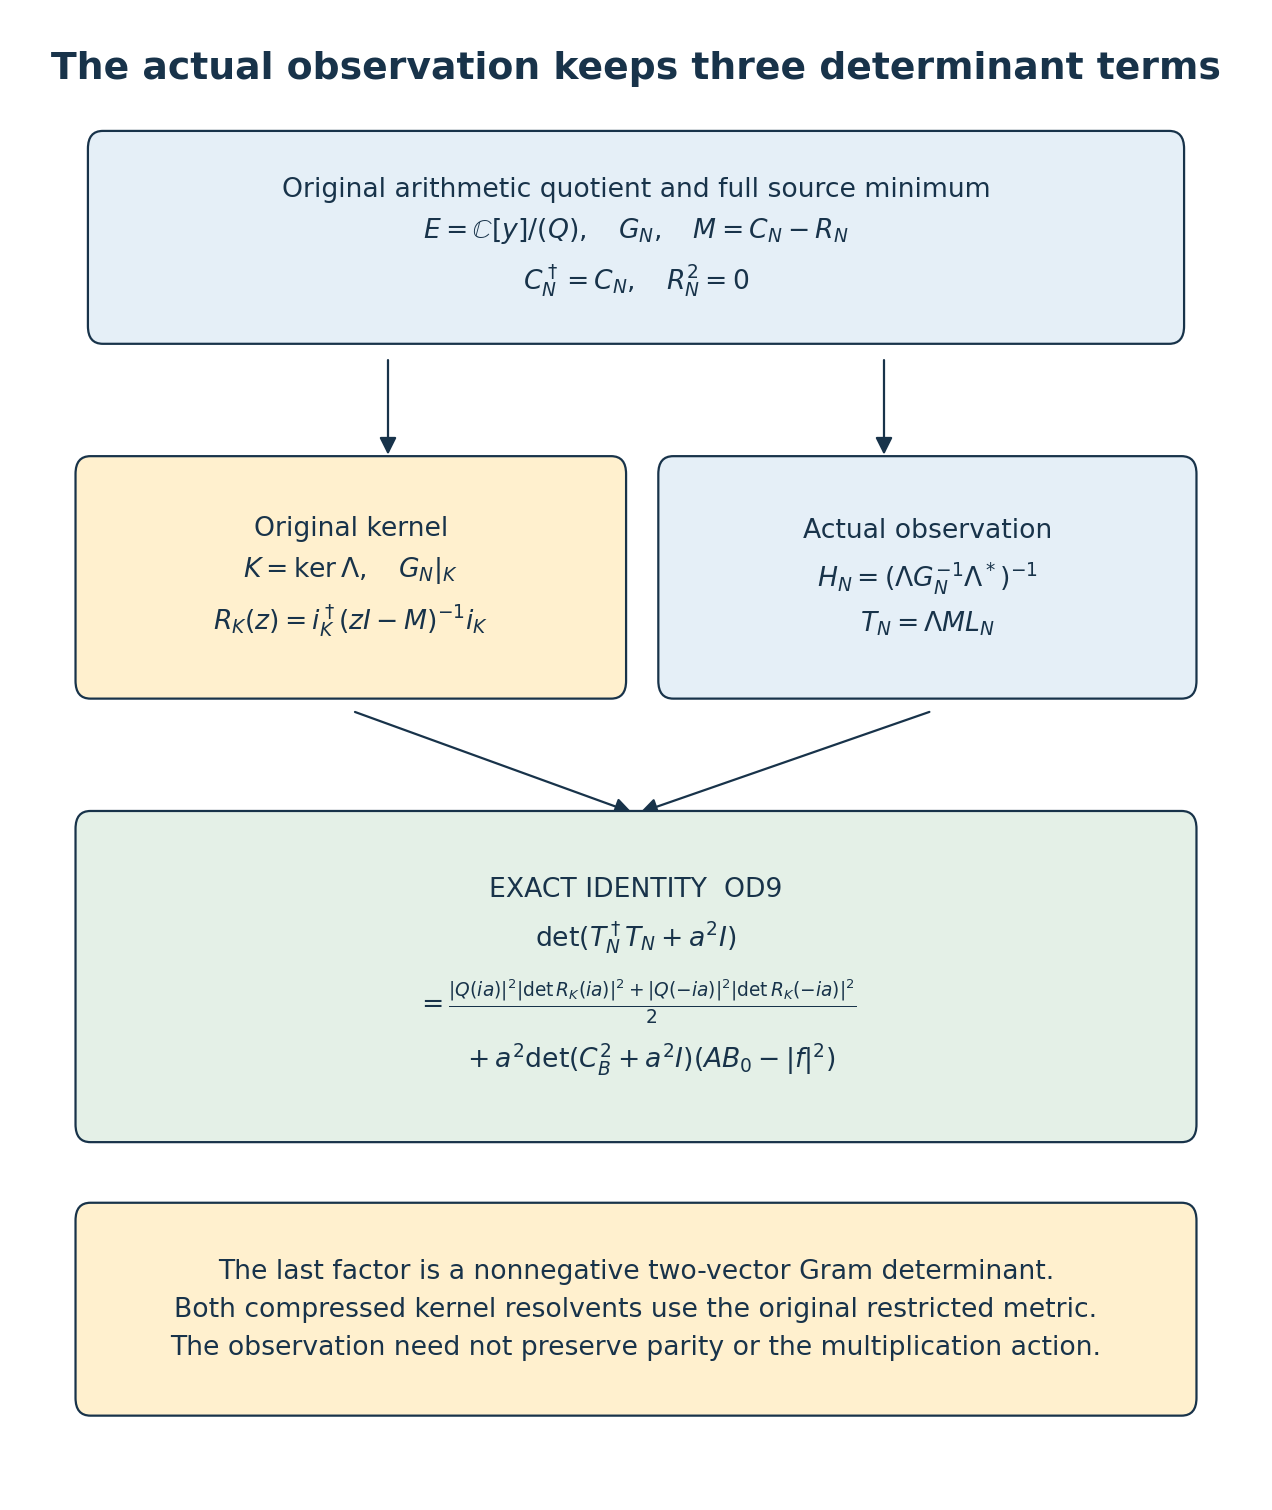
\includegraphics[width=\textwidth,height=.84\textheight,keepaspectratio]{OBSERVATION_DETERMINANT_MAP.png}
\caption{OD3--11 give the exact maps and determinant in the original attained metrics. The nonnegative term is the full boundary Gram, not an omitted phase. The two kernel resolvents retain the full root polynomial, including all multiplicities.}
\end{figure}\clearpage
\begin{figure}[p]\centering
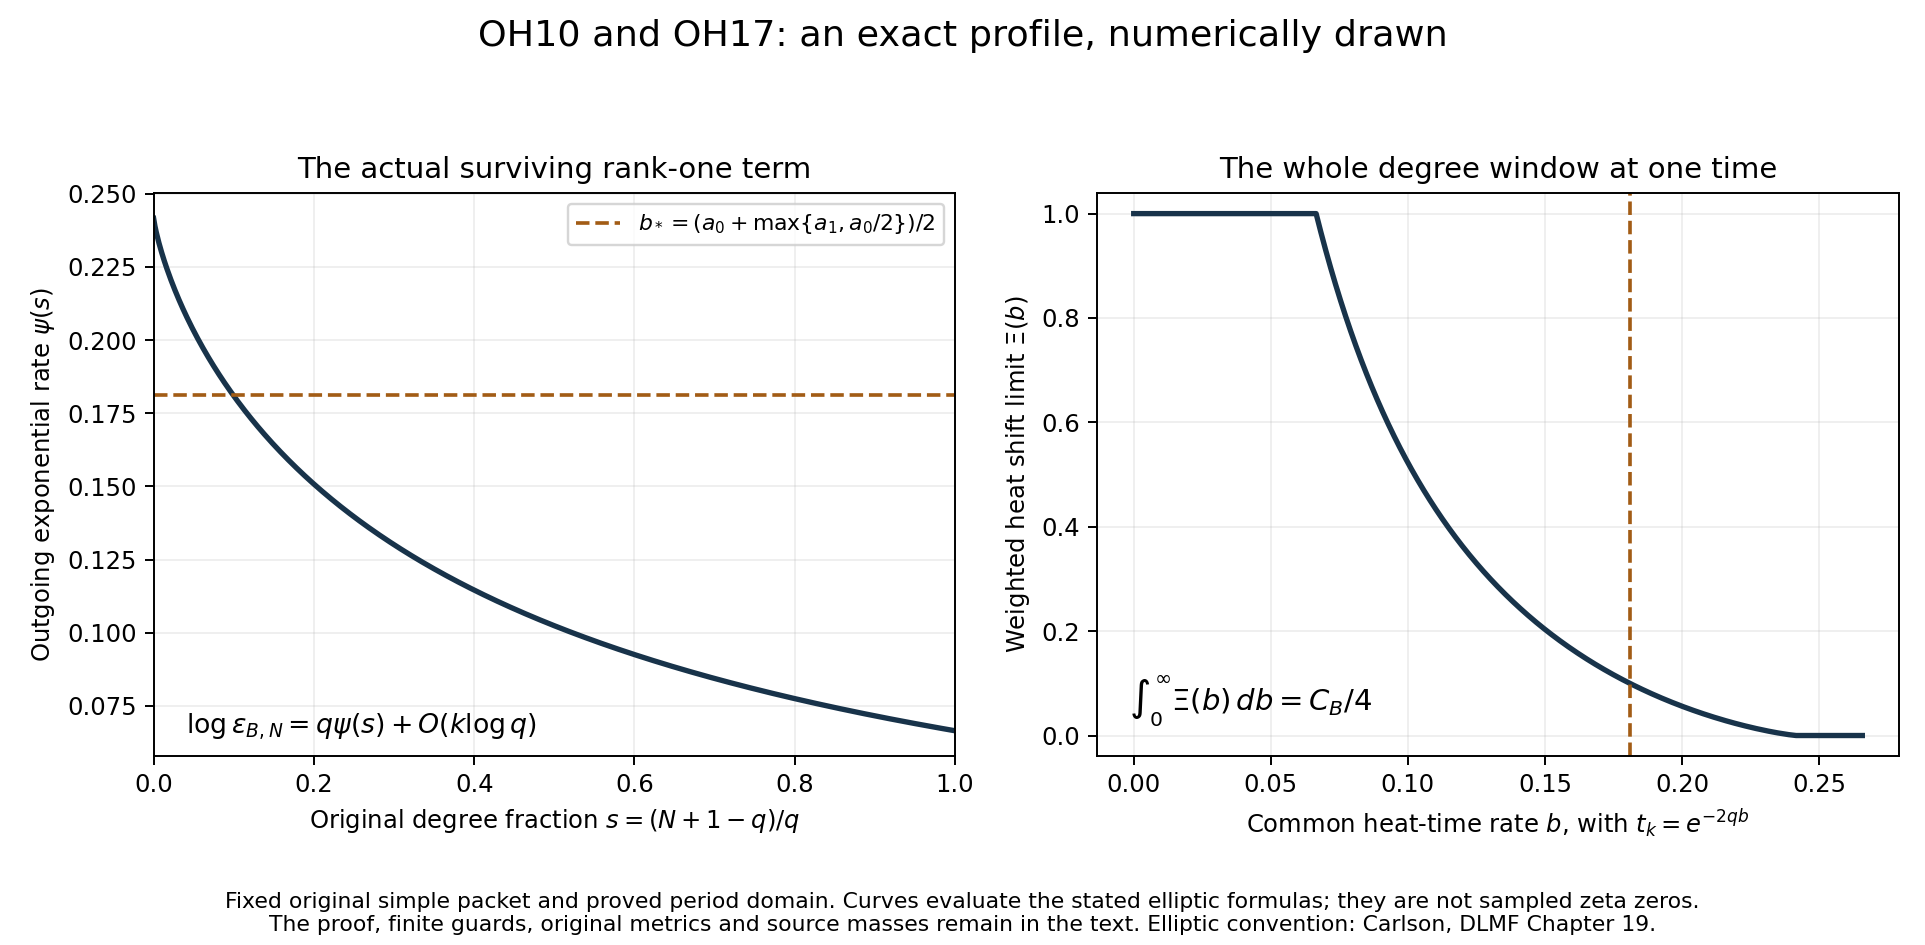
\includegraphics[width=\textwidth]{OBSERVED_HEAT_PROFILE.png}
\caption{The proved full-window profile OH8--10 and its observed heat distribution OH17. The curves are numerical renderings of exact formulas. They do not provide an effective degree threshold. The same common heat time in OH15--16 gives the four-cutoff value two. Human elliptic conventions are Carlson's DLMF Chapter 19, cited in the proof.}
\end{figure}\clearpage
\section{What is returned to the unfinished signed calculation}
OD9 is the exact receiving determinant for the original observation,
including every full-root and kernel factor. OH12 and OH18 retain the
original kernel determinant at its actual $kq$ scale. BL3--4 evaluate
a bounded two-scale logarithm, not the separate unregularized
allocations. None of these positive determinant or heat quantities
assigns the phase of $\overline{b_N^*GP_Bv}\,b_{N+1}^*GP_Bv$.
The accompanying full CP1--26 derivation keeps the original retained
class, conductor, kernel and additional conductor complement in that
signed current. Thus the next native phase calculation has these
exact receivers available without replacing its metric or source.


\appendix
\clearpage
\section*{Complete native conductor and signed complement}

This calculation derives the actual action defect on the original observation,
then passes it through the degree-eight conductor and the same attained metric.
It evaluates a signed conductor receiver on the original retained class.
The native observed current is expressed using that conductor defect and its
entire additional complement, including the full rank-one boundary term.
Every metric below keeps the original source masses. The earlier identities
NCE17 and ORE21 are inputs, rather than new results claimed here.

\section{Original domain, source and observation}
Retain a simple hypothetical actual quartet of zeros of the original zeta
source, with original multiplicity $m_0=1$, with $\rho=1/2+\delta+i\gamma$, $0<\delta<1/2$, $\gamma>2$.
Take $k\equiv1\pmod4$, $k\ge9$, $j=k-8$, $q=(k+1)^2$,
$q_-=(k-7)^2$, $c=k/2$, $c_-=j/2$, and $q-1\le N\le2q$.
The original period $\varpi$ lies in the proved size-five orbit domain.
Whenever $a_{88}\ne0$ is used, retain the stronger original domain
$|\varpi|\ge R_{\rm corner}^{\rm explicit}$ of OC71--73 \cite{CPOB}%
% BEGIN VERIFIED PUBLIC PROOF LINK
~\href{https://github.com/KokunoYumeto/zeta-function-research-reader/blob/487253b5b01851da5b9b98af4e146fecf1fab902/workbenches/splitzero-tandem/continuations/20260920-heat-literature-observed-class/HEAT_LITERATURE_AND_OBSERVED_CLASS.tex\#L1223}{[proof OB1]}%
% END VERIFIED PUBLIC PROOF LINK
{}.
Keep
\begin{equation}\tag{CP1}
 \begin{gathered}
 \chi_k(S)=\prod_{a,b=0}^k
 [S-c-(2a-k)\delta-i(2b-k)\gamma],\\
 E_k=\C[S]/(\chi_k),\qquad A_k[P]=[SP],\qquad
 v=\frac{\chi_k(S)}{(S-k\rho)\chi_k'(k\rho)},\\
 A_kv=\lambda v,\quad \lambda=k\rho,\quad
 \zeta=\lambda-c=k\delta+ik\gamma,\quad d=k\delta.
 \end{gathered}
\end{equation}
Use the physical source $dm_k=w_h^{*k}(y)\dd y$,
$w_h(y)=|(2\xi/h)(1/2+iy)|^2/(2\pi)$, at $S=c+iy$.
Let $T_N:E_k\to\mathcal P_{\le N}$ be the unique attained section,
$G=G_N$ its original positive metric, and
$b_n=[p_n]$, $\omega_n=\|p_n\|_{m_k}^2$ for the original $S$-monic
orthogonal polynomials. Thus $x^*Gy=\langle T_Nx,T_Ny\rangle_{m_k}$.
The observation is the given onto map $\Lambda:E_k\to B_k$.
Set
\begin{equation}\tag{CP2}
 \begin{gathered}
 Q=(\Lambda G^{-1}\Lambda^*)^{-1},\quad
 \Omega=\Lambda^*Q\Lambda,\quad L=G-\Omega,\\
 P_B=G^{-1}\Omega,\quad P_K=I-P_B,
 \quad w=P_Bv,\quad x=P_Kv.
 \end{gathered}
\end{equation}
Both are the original minima; $G$ first minimizes over all polynomial
relations, and $Q$ then minimizes over the complete observation kernel.
Write $e_B=w^*Gw$, $e_K=x^*Gx$, $E=v^*Gv=e_B+e_K$.
The actual current is
\begin{equation}\tag{CP3}
 \Phi_B=\frac{2\Re(\overline{B_1}B_2)}{\omega_N},\quad
 \Phi_K=\frac{2\Re(\overline{K_1}K_2)}{\omega_N},\qquad
 B_i=b_{N+i-1}^*Gw,\quad K_i=b_{N+i-1}^*Gx.
\end{equation}
The full original action formula, with its signs and monic phases, is
\begin{equation}\tag{CP4}
 A_k-cI=i\mathcal J_N+
rac{b_{N+1}b_N^*G}{\omega_N},\qquad
 \mathcal J_N^*G=G\mathcal J_N,
 \quad \|\mathcal J_N\|_G\le
 B_N:=C_{\rm mult}(h)(2N+\lfloor k/3\rfloor).
\end{equation}
Indeed multiplication of $T_Nz$ by $S$, followed by subtraction of its
leading coefficient times $p_{N+1}$, gives the compressed multiplication
by $c+iy$. Its class must then be restored by adding
$b_{N+1}b_N^*Gz/\omega_N$. The real multiplication compression is
selfadjoint, and CAI25 \cite{CPProgramme}%
% BEGIN VERIFIED PUBLIC PROOF LINK
~\href{https://github.com/KokunoYumeto/zeta-function-research-reader/blob/5992ad50c0f2a06921f1fcaded7b4e38097c0739/workbenches/splitzero-tandem/continuations/20260920-original-kernel-mixed-determinants/cumulative/09_UPDATED_JOINT_NOTE.tex\#L11282}{[proof OQC1]}%
% END VERIFIED PUBLIC PROOF LINK
{} bounds its norm through the
unchanged isometric section. This proves (CP4), including the entire
outgoing degree. In particular
$D_N=A_k^*G+GA_k-kG$ is the rank-two boundary matrix and
$\Phi_B=w^*D_Nw$, $\Phi_K=x^*D_Nx$.

\section{An explicit coefficient matrix for the observation action defect}
Retain the exact OQC coordinates: $\mathsf H$ is the original period/unit
isomorphism, $Q_0(t)=t_{++}t_{--}-t_{+-}t_{-+}$,
$Q_{\rm geom}(X)=Q_0(\mathsf H^{-1}X)$, and
\[
 \mathcal G=\mathsf H\operatorname{diag}(\gamma-i\delta,-\gamma-i\delta,
                    \gamma+i\delta,-\gamma+i\delta)\mathsf H^{-1},
 \qquad \mathcal D=\sum_{a,b=1}^4\mathcal G_{ab}X_b\partial_{X_a}.
\]
This $\mathcal G$ is the geometric action matrix; it is distinct from
the original metric $G_N$, with their exact roles displayed.
The map $\Theta_k$ of OQC7 sends the degree-$k$ quotient by
$Q_{\rm geom}$ to $E_k^\vee$ and satisfies
$\Theta_k\mathcal D=Y_k^\vee\Theta_k$, $Y_k=(A_k-cI)/i$.

Choose actual weight-zero monomials $f_\alpha=X^{\nu(\alpha)}$ whose
classes give a basis of the original invariant image in that quotient.
They exist because those monomials span that image. Let the invertible
coordinate map $S_B:B_k\to\C^{\rank\Lambda}$ be determined by
$\Lambda_0=S_B\Lambda$, whose rows are $\Theta_k[f_\alpha]$.
This defines a proved change of frame; the original $Q$ and $\Lambda$
remain in all final expressions. Define
\begin{equation}\tag{CP5}
 \begin{split}
 \eta_\alpha&=\sum_{a=1}^4\nu_a(\alpha)\mathcal G_{aa},\\
 (\Xi_0z)_\alpha&=
 \Theta_k\left[\sum_{a\ne b}\nu_a(\alpha)\mathcal G_{ab}
 X^{\nu(\alpha)-e_a+e_b}\right](z),\\
 Z_B&=S_B^{-1}\operatorname{diag}(\eta_\alpha)S_B,
 \qquad \Xi=S_B^{-1}\Xi_0.
 \end{split}
\end{equation}
Terms with $\nu_a=0$ are zero before the monomial is formed.
Then the full exact action and its kernel restriction are
\begin{equation}\tag{CP6}
 \boxed{\Lambda Y_k=Z_B\Lambda+\Xi,\qquad
             \Lambda Y_k|_{\ker\Lambda}=\Xi|_{\ker\Lambda}.}
\end{equation}
To prove this, differentiate each chosen monomial. The diagonal terms
give $\eta_\alpha f_\alpha$ and the remaining terms are exactly (CP5).
Their weights differ from zero by $b-a$ modulo five; since
$1\le a,b\le4$, only $a=b$ retains weight zero. Hence the original
Reynolds average kills precisely these off-diagonal terms. The equality
$\Theta_k\mathcal D=Y_k^\vee\Theta_k$ proves (CP6) on $E_k$.
This gives the matrix of OQC22--23 before any phase is estimated.
Changing representatives changes both displayed summands compatibly;
their sum is the fixed original map $\Lambda Y_k$.

With $b=\Lambda v$ and $Y_kv=(k\gamma-ik\delta)v$, (CP6) gives
$\Xi v=((k\gamma-ik\delta)I-Z_B)b$ exactly. On the attained lift,
$\Lambda Y_kw=(k\gamma-ik\delta)b-\Xi x$.
Pair with the original $b^*Q$ and use
$\Re(iu)=-\Im u$ to obtain the concrete phase-defect formula
\begin{equation}\tag{CP7}
 \boxed{\Phi_B=2d e_B+2\Im(b^*Q\Xi x).}
\end{equation}
The imaginary part retains the actual relative complex phase. The
commutator in (CP5) has not been replaced by its rank or its modulus.

\section{The literal degree-eight conductor and its derivative}
Let the original OQC product of four nonidentity orbit quadrics have
the retained biform coefficients $a_{uv}$, $0\le u,v\le8$.
Its original contraction is the onto map $C:E_k\to E_j$ given by
\begin{equation}\tag{CP8}
 \begin{split}
 (\mathcal T_AP)(S_-)&=\sum_{u,v=0}^8a_{uv}P(S_-+\sigma_{uv}),\\
 \sigma_{uv}&=4+(2u-8)\delta+i(2v-8)\gamma,\\
 C[P]&=[\mathcal T_AP],\qquad
 C_1[P]=\left[\sum_{u,v=0}^8(\sigma_{uv}-4)a_{uv}
                         P(S_-+\sigma_{uv})\right].
 \end{split}
\end{equation}
Both maps are well defined. At every lower grid root, its translate
by any $\sigma_{uv}$ is an upper grid root. A polynomial divisible by
$\chi_k$ therefore maps to zero at every lower root; those lower roots
are distinct, proving divisibility by $\chi_j$ in both cases.
The original injection by the degree-eight orbit product in OQC19
duals to surjectivity of $C$, and gives
$\ker\Lambda\subset\ker C$. Thus there is a unique onto map
$D:B_k\to E_j$ with $C=D\Lambda$.
These are the actual OQC/OB maps, including their original coefficients.

Termwise multiplication by $S_-+\sigma_{uv}$ proves the full defect
\begin{equation}\tag{CP9}
 \boxed{C(A_k-cI)-(A_j-c_-I)C=C_1.}
\end{equation}
In the physical $Y$ coordinate this is
$CY_k-Y_jC=C_1/i$. It is exactly the dual of the derivative of
the degree-eight product in OQC22, with its centering factor retained.
For the same original terminal cardinal class, evaluating at all lower
grid roots proves
\begin{equation}\tag{CP10}
 Cv=a_{88}v_-,\qquad C_1v=8(\delta+i\gamma)a_{88}v_-,\qquad
 v_-=\frac{\chi_j(S_-)}{(S_--j\rho)\chi_j'(j\rho)}.
\end{equation}
Every evaluation vanishes except the upper terminal root. It can be
reached from a lower root only with the terminal lower root and
$(u,v)=(8,8)$, proving both scalars, including the complex phase.
In particular (CP9) is a computed defect, rather than an assumed
intertwining of the two multiplication operators.

\section{The exact nested minimum and its full additional complement}
Define the conductor metric through the \emph{same original} $G_N$ by
\begin{equation}\tag{CP11}
 H_C=(D Q^{-1}D^*)^{-1}=(C G^{-1}C^*)^{-1},\qquad
 P_C=G^{-1}C^*H_CC,\quad u=P_Cv,\quad t=(P_B-P_C)v.
\end{equation}
The equality of inverse matrices follows from
$Q^{-1}=\Lambda G^{-1}\Lambda^*$ and $C=D\Lambda$.
All inverses are positive because the indicated maps are onto.
The vector $G^{-1}C^*H_Cb_C$ is the unique minimum-norm lift of
$b_C\in E_j$: it has image $b_C$ and is orthogonal to $\ker C$.
Thus $P_C$ is the $G$-orthogonal projection onto $(\ker C)^{\perp_G}$.
Since $\ker\Lambda\subset\ker C$, these orthogonal projections satisfy
$P_BP_C=P_CP_B=P_C$. Consequently
\begin{equation}\tag{CP12}
 \begin{gathered}
 v=u+t+x,\qquad u\perp_G t\perp_G x\perp_G u,\\
 t\in\mathcal T_N:=\ker C\cap(\ker\Lambda)^{\perp_G},\\
 e_C=(Cv)^*H_C(Cv),\quad e_T=t^*Gt,\quad
 e_B=e_C+e_T,\quad E=e_C+e_T+e_K.
 \end{gathered}
\end{equation}
On the proved size-five orbit, the original exact ranks are
$\rank\Lambda=k^2-6k+17$ and $\rank C=q_-=(k-7)^2$.
Their actual difference, for every allowed $k\ge9$, is
\begin{equation}\tag{CP13}
 \boxed{\begin{gathered}\dim\mathcal T_N=(k^2-6k+17)-(k-7)^2=8k-32,\\
 \dim\ker\Lambda=(k+1)^2-(k^2-6k+17)=8k-16.\end{gathered}}
\end{equation}
The first dimension is a kernel dimension of the onto map $D$.
It is not an allocation of norm or current according to dimension.

Here are complete small-block coordinates, avoiding a further implicit
choice of complement. Let $I$ be any fixed injective frame of
$\ker\Lambda$, and choose $J$ such that $[I,J]$ is a frame of $\ker C$.
Put
\begin{equation}\tag{CP14}
 \begin{split}
 H_K&=I^*GI,\qquad
 J_N=J-IH_K^{-1}I^*GJ,\\
 H_T&=J_N^*GJ_N=J^*GJ-J^*GIH_K^{-1}I^*GJ,\\
 \alpha&=H_K^{-1}I^*Gv,\qquad
 \beta=H_T^{-1}J_N^*Gv,\qquad x=I\alpha,\quad t=J_N\beta.
 \end{split}
\end{equation}
$J_N$ is in $\ker C$, orthogonal to $\ker\Lambda$ and injective:
if $J_Nz=0$, then $Jz\in\operatorname{im}I$, contradicting the
independence of $[I,J]$ unless $z=0$. Its dimension is (CP13), so it
is a frame of $\mathcal T_N$. The last two formulas are the two exact
orthogonal projections, proving (CP14). Thus the additional metric is
the displayed full Schur complement, with every cross block retained.

\section{The native phase receiver and the complete boundary term}
Let $b_C=Cv=a_{88}v_-$. Define the actual complex leakage scalars
\begin{equation}\tag{CP15}
 \mathcal L_{CK}=b_C^*H_C C_1I\alpha,\qquad
 \mathcal L_{TK}=\beta^*J_N^*G(A_k-cI)I\alpha.
\end{equation}
Then the original observed current is exactly
\begin{equation}\tag{CP16}
 \boxed{\Phi_B=2d(e_C+e_T)-2\Re(\mathcal L_{CK}+\mathcal L_{TK}).}
\end{equation}
Indeed $(A_k-cI)w=\zeta v-(A_k-cI)x$ and $w^*Gv=e_B$.
The row of $u$ is $u^*G=b_C^*H_CC$, while $Cx=0$.
Equation (CP9) therefore gives
$u^*G(A_k-cI)x=b_C^*H_CC_1x=\mathcal L_{CK}$.
The remaining row is $t^*G(A_k-cI)x=\mathcal L_{TK}$.
Taking twice the real part proves (CP16), on the same metric and class
as (CP3), without replacing any response by its absolute value.

In particular, set $T_i=b_{N+i-1}^*Gt$. The full boundary in (CP4)
gives the further exact expansion
\begin{equation}\tag{CP17}
 \mathcal L_{TK}=i\,t^*G\mathcal J_Nx+
                    \frac{\overline{T_2}K_1}{\omega_N},
 \qquad
 \left|\Phi_B-\left[2d e_B-2\Re\left(
 \mathcal L_{CK}+\frac{\overline{T_2}K_1}{\omega_N}\right)\right]\right|
 \le2B_N\sqrt{e_Te_K}.
\end{equation}
The error is the real scalar $2\Im(t^*G\mathcal J_Nx)$.
Cauchy--Schwarz in the original metric and (CP4) give the displayed
finite bound. The rank-one boundary term is retained exactly and
has not been bounded by the norm of the full nonnormal action.
For $N\le2q$, $B_N=O_h(q)$. No bound on $T_2K_1$ is inferred
from that fact or from (CP13).

All complementary currents can be recovered without losing a mixed term.
For $a,b\in\{u,t,x\}$ put $h_{ab}=a^*G(A_k-cI)b$.
The eigenclass equation proves
\begin{equation}\tag{CP18}
 \sum_bh_{ab}=\zeta e_a,\quad
 \Phi_a=2\Re h_{aa}=2d e_a-2\Re\sum_{b\ne a}h_{ab},\quad
 \Phi_{ab}=2\Re(h_{ab}+h_{ba})\quad(a\ne b).
\end{equation}
Here the sum of the three diagonal currents and all three unordered
mixed currents is $2dE$. Moreover
$\Phi_B=\Phi_u+\Phi_t+\Phi_{ut}$,
$\Phi_K=\Phi_x$, and
$\Phi_{\times}=\Phi_{ux}+\Phi_{tx}$.
The complete conductor row is
\[
 h_{ux}=b_C^*H_CC_1x,\qquad h_{ut}=b_C^*H_CC_1t,\qquad
 h_{uu}=\zeta e_C-h_{ut}-h_{ux}.
\]
Thus even the native conductor component alone retains its two original
action defects. Neither has been declared zero.

\section{An evaluated signed conductor receiver and its metric map}
For clarity, the lower original arithmetic metric is a second specified
metric: $G^-_N$ is the attained metric on $E_j$ from degree at most $N$
in the unchanged source $m_j=w_h^{*j}$ at $c_-+iy$.
Define $E_C^-=b_C^*G^-_Nb_C=|a_{88}|^2v_-^*G^-_Nv_-$.
The lower current and the full degree-eight defect on the original
retained class have the exact positive values
\begin{equation}\tag{CP19}
 \begin{split}
 2\Re[b_C^*G^-_N(A_j-c_-I)b_C]&=2j\delta E_C^-,\\
 2\Re[b_C^*G^-_NC_1v]&=16\delta E_C^-,\\
 2\Re[b_C^*G^-_NC(A_k-cI)v]&=2k\delta E_C^-.
 \end{split}
\end{equation}
These follow from (CP9)--(CP10) and the actual lower eigenvalue
$j\rho$; the complex coefficient in the middle line is precisely
$8(\delta+i\gamma)$ before its real part is taken.
For the \emph{actual observed lift} $w$, define
$\mathfrak I_C^-(w)=2\Re[b_C^*G^-_NC(A_k-cI)w]$. Its exact value is
\begin{equation}\tag{CP20}
 \mathfrak I_C^-(w)=2k\delta E_C^-
                      -2\Re[b_C^*G^-_NC_1x].
\end{equation}
An explicit bound for this remaining complex term follows from the
original full-polynomial comparison and the Gamma translation formula.
Let $\ell_{k,N}$ be the unchanged CAI16--18 lower constant. For $j\ge3$
put $A_{j,N}^+=A_j$ and $\ell_{j,N}^-=a_j/[1+4(N+25)^2]^{25}$,
with the unchanged CAI16--18 constants. At the single admissible value
$k=9$, $j=1$, define $A_{1,N}^+$ and $\ell_{1,N}^-$ as the largest
and smallest eigenvalues of
$H_{\sigma,N}^{-1/2}H_{w_h,N}H_{\sigma,N}^{-1/2}$, where the two
Grams are the complete degree-$N$ original monomial Grams.
They are finite and strictly positive: the sources have all moments,
and each gives positive norm to every nonzero polynomial. For $w_h$ this
follows because $2\xi/h$ is a nonzero entire function with isolated zeros.
The Rayleigh quotient proves the two full-form inequalities at this
finite exception. Thus no lower comparison for convolution order one
is inferred from the order-three CAI theorem. Put
\begin{equation}\tag{CP21}
 \begin{split}
 z_{uv}&=(2v-8)\gamma-i(2u-8)\delta,\\
 \mathcal T_N(z)&=\exp(1)(N+1)(2N+1)^{(|z|+1)/2},\\
 L_{1,N}&=\sqrt{A_{j,N}^+/\ell_{k,N}}
       \sum_{u,v=0}^8|\sigma_{uv}-4|\,|a_{uv}|\mathcal T_N(z_{uv}),\\
 L_{0,N}&=\sqrt{A_{j,N}^+/\ell_{k,N}}
       \sum_{u,v=0}^8|a_{uv}|\mathcal T_N(z_{uv}).
 \end{split}
\end{equation}
These constants are positive, finite and retain every coefficient.
The original translation estimate OB11 follows from the
Meixner--Pollaczek generating function \cite{CPDLMF18}: translation
multiplies it by $e^{z\arctan t}$. On $|t|=N/(N+1)$ its first
$N+1$ coefficients have modulus at most
$\exp(1)(2N+1)^{|z|/2}$. The original coefficient weights have each
gap-$l$ ratio at most $\sqrt{2l+1}$; summing their $N+1$ diagonals
gives exactly $\mathcal T_N$. Thus each summand in (CP8) has that
norm from the Gamma source at $c$ to that at $c_-$.
The whole-polynomial bounds
$\ell_{k,N}\|P\|_\sigma^2\le\|P\|_{m_k}^2$ and
$\|P\|_{m_j}^2\le A_{j,N}^+\|P\|_\sigma^2$, followed by the actual
lower minimum, prove
\begin{equation}\tag{CP22}
 \|C_1z\|_{G^-_N}\le L_{1,N}\|z\|_G,\qquad
 \|Cz\|_{G^-_N}\le L_{0,N}\|z\|_G.
\end{equation}
Apply this to the attained representative $T_Nz$; both images have
degree at most $N$, so no new target cutoff has been substituted.
Consequently
\begin{equation}\tag{CP23}
 |\mathfrak I_C^-(w)-2k\delta E_C^-|
 \le2L_{1,N}\sqrt{E_C^-e_K},\qquad
 \log^+L_{1,N}=O_{h,\varpi}(k+\log q).
\end{equation}
The last bound uses the original CAI constants, fixed degree-eight
coefficients and fixed shifts, with $N\le2q$.

The exact original metric map between this receiver and the native one is
\begin{equation}\tag{CP24}
 \Phi_B-\mathfrak I_C^-(w)
 =2\Re\{b^*(Q-D^*G^-_ND)\Lambda(A_k-cI)w\},
 \qquad G^-_N\preceq L_{0,N}^2H_C.
\end{equation}
The equality is substitution of $C=D\Lambda$, not an identification
of the two metrics. For the inequality, minimize (CP22) over the
unchanged affine fibre $Cz=b_C'$; the minimum is $b_C'^*H_Cb_C'$.
It holds for every $b_C'$, proving the Loewner comparison.
The exact identity also keeps the native residual as the full matrix
$Q-D^*G^-_ND$; its current is not assigned a sign.

For a quantitative relative size in (CP23), let
$\Delta=q-q_-=16k-48$, $R=k\sqrt{\delta^2+\gamma^2}$,
$R_-=j\sqrt{\delta^2+\gamma^2}$,
$B_-=2q_-/\delta+2+\pi/2$ and
\[
 \begin{gathered}
 g_N=\{1+B_-^2[R_-^2+4(N+3)^2]\}^{-1},\quad
 D_k(S)=\frac{\chi_k(S)}{\chi_j(S-8\rho)},\\
 V_N=\frac{\mathcal T_{N-\Delta}(-8\gamma+8i\delta)^2
                   [2(N+1)+R]^{2\Delta}}{|D_k(k\rho)|^2}.
 \end{gathered}
\]
The actual reverse cardinal lift is
$D_k(S)P_-(S-8\rho)/D_k(k\rho)$. Its degree is at most $N$ when
$\deg P_-\le N-\Delta$, and its original Gamma squared norm is at
most $V_N$ times that lower norm. The consecutive residual estimate
OB4--9 gives
$E_-^\sigma(N)\ge g_N^\Delta E_-^\sigma(N-\Delta)$.
These are the original full residuals, including all lower relations.
Using the two original arithmetic/Gamma comparisons proves
\begin{equation}\tag{CP25}
 \frac{E}{E_C^-}\le
 R_N^{\rm card}:=\frac{A_k V_N g_N^{-\Delta}}
                       {\ell_{j,N}^-|a_{88}|^2},\qquad
 \log^+R_N^{\rm card}=O_{h,\varpi}(k\log q).
\end{equation}
For the last assertion the complete product for $D_k(k\rho)$ has
$\Delta$ factors of modulus at least $2(k-7)\delta$ (OB10), while
$-\log g_N=O_h(\log q)$, $\Delta=O(k)$, and the translations have
fixed exponents. Every displayed source comparison costs $O_h(k+\log q)$.
Thus (CP23) yields the finite signed interval
\begin{equation}\tag{CP26}
 \left|\frac{\mathfrak I_C^-(w)}{E_C^-}-2k\delta\right|
 \le2L_{1,N}\sqrt{R_N^{\rm card}}\sqrt{e_K/E},\qquad
 \log^+\!\left(2L_{1,N}\sqrt{R_N^{\rm card}}\right)
                         =O_{h,\varpi}(k\log q).
\end{equation}
This is a quantified size bound on the retained complex error; it
does not determine its sign. The native current remains (CP16)--(CP18)
with the exact comparison (CP24). In particular neither the full
$8k-32$ complement nor the derivative conductor is removed from it.



\clearpage
\section*{Complete general-family collision and native receivers}



\section{Inputs, coordinates, and scope}
The input is the supplied \emph{General-family control: complete new proofs},
20 September 2026, specifically T1--T31, S1--S26, Q1--Q25,
C1--C13, H1--H9 and F1--F7. Its companion is
\emph{General-family control: multiplicities, collisions, source sections,
and all mixed minima}. Both documents were read in full. Their hashes,
exact reading coverage and the limited literature-index search appear in
the accompanying reading ledger. This note gives independent proofs of
the assigned tensor-length, collision and source-minimum calculations and
extends their explicit receivers. It does not assign either document a
human author absent supporting attribution.

Every Hermitian scalar product below is conjugate-linear in its first
argument. A star means the conjugate transpose in the specified original
coefficient coordinates; a dagger means the adjoint for the stated
metrics. Matrix square roots and pseudoinverses are auxiliary coordinate
operations, with their composite maps identified below. None changes the
original source measure or the arithmetic quotient.

For factor $i$, keep
\[
h_i(s)=\prod_{\rho\in Z_i}(s-\rho)^{m_{i,\rho}},\qquad
d_{i,\rho}=m_{i,\rho}-1,
\quad E_i=\C[s]/h_i.
\]
Use the full divided jets $P^{(j)}(\rho)/j!$. Multiplication by the
physical unit $u_i=j_{h_i}(2\xi/h_i)$ is the complete triangular matrix
$U_i$. On admitted arithmetic divisors, all its constant local
coefficients are nonzero. The inverse uses the entire finite inverse
series, and the physical metric is transported by $(U_i^{-1})^*G_iU_i^{-1}$.
Thus every calculation in polynomial jets returns through $U_i$ without
discarding higher derivatives. The physical-source statements concern
these admitted divisors, not arbitrary coefficient values assigned to zeros.

\section{The complete tensor-length calculation}
For $0<\eta\le1$ and positive $a_{i,\rho}$, put
\[
\|z^j\|^2=a_{i,\rho}(j!)^2\binom{d_{i,\rho}}j\eta^{2j}.
\tag{GF1}
\]
On each primary block, multiplication $N=M_z$ has
$N^\dagger z^j=\eta^2j(d-j+1)z^{j-1}$. This follows by taking the
ratio of the two adjacent diagonal metric entries. With
$E=N/\eta$, $F=N^\dagger/\eta$, $H=[F,E]$, direct application to
$z^j$ gives $H z^j=(d-2j)z^j$, $[H,E]=-2E$, $[H,F]=2F$.
These identities retain the whole local algebra, including its last jet.

For an ordered root tuple $\boldsymbol\rho$, write
$\kappa=\sum_i\rho_i$, $D=\sum_i d_{i,\rho_i}$,
$A=\prod_i a_{i,\rho_i}$ and $R=\sum_i z_i$.
The coefficient of the top ordered monomial in $R^D$ is
$D!/\prod_i d_{i,\rho_i}!$, so it is nonzero. Also $R^{D+1}=0$.
Consequently the original sum-cyclic algebra has polynomial
\[
\chi(S)=\prod_\kappa(S-\kappa)^{D_\kappa+1},\qquad
D_\kappa=\max_{\sum\rho_i=\kappa}\sum_i d_{i,\rho_i}.
\tag{GF2}
\]
This maximum is taken after all actual additive collisions are identified.
The cyclic injection $\beta$ takes $P$ to $P(\sum_i s_i)$.

Define $W_{\kappa,D}$ to be the sum of $A$ over every ordered tuple
with this centre and length, and put
$S_{\kappa,j}=\sum_DW_{\kappa,D}\binom Dj$.
The multinomial coefficient in $R^j$ cancels the factorials in (GF1),
giving the exact norm $A(j!)^2\eta^{2j}\binom Dj$.
Different total degrees are orthogonal. Hence
\[
G_{\mathrm{cyc}}\big|_{\kappa,j}
=(j!)^2\eta^{2j}S_{\kappa,j}.
\tag{GF3}
\]

\begin{proposition}[Every adjoint-leakage direction]
Let $A_\Sigma$ be multiplication by $\sum_i s_i$, and let $A$ be
multiplication by $S$ on the cyclic algebra. With $\Pi=\beta\beta^\dagger$,
define $Z=(I-\Pi)A_\Sigma^\dagger\beta$. Then
\[
Z^\dagger Z\big|_{\kappa,j}
=\eta^2\frac{S_{\kappa,j-1}}{S_{\kappa,j}}
\Var_{\pi_{\kappa,j-1}}(D),\qquad
\pi_{\kappa,j-1}(D)=\frac{W_{\kappa,D}\binom D{j-1}}{S_{\kappa,j-1}}
\tag{GF4}
\]
for $j\ge1$, and its value at $j=0$ is zero. If the largest two distinct
retained lengths are $D_1>D_2$, then $\rank Z_\kappa=D_2+1$.
If there is only one distinct length, the rank is zero.
\end{proposition}
\begin{proof}
The tensor commutators, or direct differentiation of its multinomial
expansion, give $R^\dagger R^j=\eta^2j(D-j+1)R^{j-1}$.
Projection onto the common coefficient of degree $j-1$ therefore subtracts
the mean of $\eta^2j(D-j+1)$ with probabilities $\pi_{\kappa,j-1}$.
The raw squared residual is
\[
\eta^4j^2((j-1)!)^2\eta^{2j-2}
S_{\kappa,j-1}\Var_{\pi_{\kappa,j-1}}(D).
\]
Dividing by the input norm in (GF3) proves (GF4). The output degrees
are distinct for distinct $j$, so the resulting operator is diagonal.
The variance is positive exactly when two different lengths are at
least $j-1$, which is equivalent to $1\le j\le D_2+1$.
In particular no unnamed additional leakage directions are left.
\end{proof}

The bound follows in the same probability space. Set $X=D-j+1$.
Then $0\le X\le D_\kappa-j+1$ and
$EX=jS_{\kappa,j}/S_{\kappa,j-1}$. Thus
\[
\|Z_\kappa\|^2\le
\max_j\eta^2j\frac{\Var X}{EX}
\le\frac{\eta^2(D_\kappa+1)^2}{4}.
\tag{GF5}
\]

\begin{proposition}[The minimal reducing enlargement]
Let $1_D$ be the vector equal to $1$ in all labelled tuple blocks of
length $D$, and zero in the others at the same centre. The subspace
generated from $\im\beta$ by the action and its adjoint is exactly
\[
\mathscr W_\kappa=
\bigoplus_{D:W_{\kappa,D}>0}\operatorname{span}
\{R^j1_D:0\le j\le D\}.
\tag{GF6}
\]
Its dimension is $\sum_D(D+1)$. The projection to the original cyclic
coordinate is
\[
v_{\kappa,j}=
\frac{\sum_DW_{\kappa,D}\binom Dj u_{D,j}}{S_{\kappa,j}}.
\tag{GF7}
\]
\end{proposition}
\begin{proof}
On the direct sum of the top chains the explicit operator
$\mathfrak C=H^2+2H+4EF$ has value $D(D+2)$ on the chain of length $D$.
Indeed on degree $j$ its value is
$(D-2j)^2+2(D-2j)+4j(D-j+1)=D(D+2)$.
Polynomial interpolation in these distinct integers gives the projector
\[
\prod_{D'\ne D}
\frac{\mathfrak C-D'(D'+2)I}{D(D+2)-D'(D'+2)}.
\]
It extracts $1_D$ from the cyclic constant vector. Multiplication by
$R$ obtains its entire chain. Conversely every such chain is invariant
under $R$ and $R^\dagger$, so no other directions are generated.
If several centres occur, their complete primary projectors are
polynomials in $A_\Sigma$; on this orthogonal primary decomposition
the adjoint preserves the same blocks. This justifies applying the
argument at each centre separately. Formula (GF7) is the orthogonal
projection for the actual diagonal norms (GF3).
\end{proof}

\section{Every simultaneous collision and jet-scale exponent}
The fixed-$\eta$ exponents C7--C10 of the input are correct. The finite
algorithm C11 can, for two channels, be evaluated completely as follows.
Let $e\ge f\ge1$, $u=S-\kappa_0$, and retain
\[
\overline E_z=\C[u]/[u^e(u-z)^f].
\]
The input polynomial basis is $1,u,\ldots,u^{e+f-1}$, and the output
is the pair of all divided jets at $0$ and $z$.
The coefficient translation from $S$ to $u$ is triangular of determinant
one, with a bounded inverse for fixed $\kappa_0$.
The evaluation matrix has rows
\[
(E_z)_{0,j;n}=\delta_{jn}\ (j<e),\qquad
(E_z)_{1,j;n}=\binom nj z^{n-j}\ (j<f,n\ge j),
\tag{GF8}
\]
and all other entries are zero. Give derivative level $j$ the retained
positive weight $\alpha_{a,j}|z|^{2aj}$, where the constants
$\alpha_{a,j}>0$ are fixed, and $a\ge0$. Equivalently
$\eta=|z|^a$ in the jet metric. Multiplication of rows by the fixed
$\sqrt{\alpha_{a,j}}$ leaves all the exponents below unchanged.
No assertion about leading constants in unspecified metrics is made.

Write singular values in decreasing order. An exponent list
$\lambda_1\le\cdots\le\lambda_{e+f}$ means that the corresponding
singular values are bounded above and below by positive constants
times $|z|^{\lambda_i}$, for fixed $a$ and small nonzero $z$.

\begin{theorem}[Closed two-regime formula]
For $0\le a\le1$, the complete ordered exponent list is
\[
\boxed{\ 0,a,\ldots,(e-1)a;\quad
e-f+2r-1+a(f-r),\quad r=1,\ldots,f.\ }
\tag{GF9}
\]
For $a\ge1$, let $j_1\le\cdots\le j_{e+f}$ be the sorted multiset
$\{0,\ldots,e-1\}\cup\{0,\ldots,f-1\}$. Then
\[
\boxed{\lambda_r=r-1+(a-1)j_r,\quad 1\le r\le e+f.}
\tag{GF10}
\]
The only possible transition is $a=1$, where both formulas are
$0,1,\ldots,e+f-1$. At $a=0$, (GF9) gives $e$ noncollapsing singular
values and exponents $e-f+1,e-f+3,\ldots,e+f-1$ for the other $f$.
\end{theorem}
\begin{proof}
Put $t=|z|$. The phase of $z$ is removable by unitary diagonal row and
column matrices, since each nonzero entry has phase $z^{n-j}$.
For $a\le1$, subtract the first-block columns from the second-block
rows. The coefficient used to subtract derivative level $n$ from
second-block derivative $j$ is
$\binom nj t^{(1-a)(n-j)}$ times its retained unit phase. These row
operations and their inverses are uniformly bounded as $t\downarrow0$.
The matrix becomes
\[
\diag(1,t^a,\ldots,t^{(e-1)a})\oplus B_{a,t},\quad
(B_{a,t})_{j,c}=\binom{e+c}j
t^{e+c+(a-1)j},\quad 0\le j,c<f.
\tag{GF11}
\]
The smallest exponent of an $r$-minor of the second block is achieved
by columns $0,\ldots,r-1$ and rows $f-r,\ldots,f-1$; it is
\[
\nu_r=r(e-f+r)+\frac{ar(2f-r-1)}2.
\tag{GF12}
\]
Its coefficient is nonzero. To see this, put $b=f-r$, factor
$(e+c)!/(e+c-b)!$ from column $c$ and $1/(b+i)!$ from row $i$.
The remaining polynomial in column variable $e+c-b$ is its falling
factorial of degree $i$. Its determinant is the classical Vandermonde
\cite{GFVandermonde} at the
consecutive integers, equal to $\prod_{\ell=1}^{r-1}\ell!$.
All other minors have at least (GF12)'s exponent by the row and column
index sums.

The squared Hilbert--Schmidt norm of the $r$th exterior matrix is the
sum of the squared moduli of its minors. Positive squared coefficients
cannot cancel. Thus it is comparable to $t^{2\nu_r}$. The largest
exterior singular value, which is the product of the first $r$
singular values, is within a fixed dimension factor of that norm.
Consecutive ratios therefore give exponents
$\nu_r-\nu_{r-1}=e-f+2r-1+a(f-r)$.
Their first value exceeds $(e-1)a$ by
$e-f+1-a(e-f)\ge1$, so the concatenated list (GF9) is indeed ordered.

For $a\ge1$, a nonzero $r$-minor of (GF8), after row weighting, has
exponent
\[
\sum_{n\in J}n+(a-1)\sum_{i\in I}j_i.
\tag{GF13}
\]
This is at least $r(r-1)/2+(a-1)\sum_{i=1}^rj_i$.
Choose the $r$ lowest derivative levels from the two channels, breaking
ties so that the selected rows at each channel form an initial segment.
Choose columns $0,\ldots,r-1$. Its confluent evaluation determinant
is a nonzero constant times $z^{e'f'}$, where $e'+f'=r$ are the selected
initial-segment lengths. It can also be obtained by the preceding
column elimination, so nonvanishing requires no outside result.
This achieves the lower exponent in (GF13). The same exterior-norm
argument gives (GF10) by consecutive differences. Its values increase
because both $r$ and the $j_r$ increase. This proves every exponent.
\end{proof}

The determinant exponent throughout both regimes is
\[
ef+\frac a2\{e(e-1)+f(f-1)\}.
\tag{GF14}
\]
\begin{figure}[htbp]
\centering
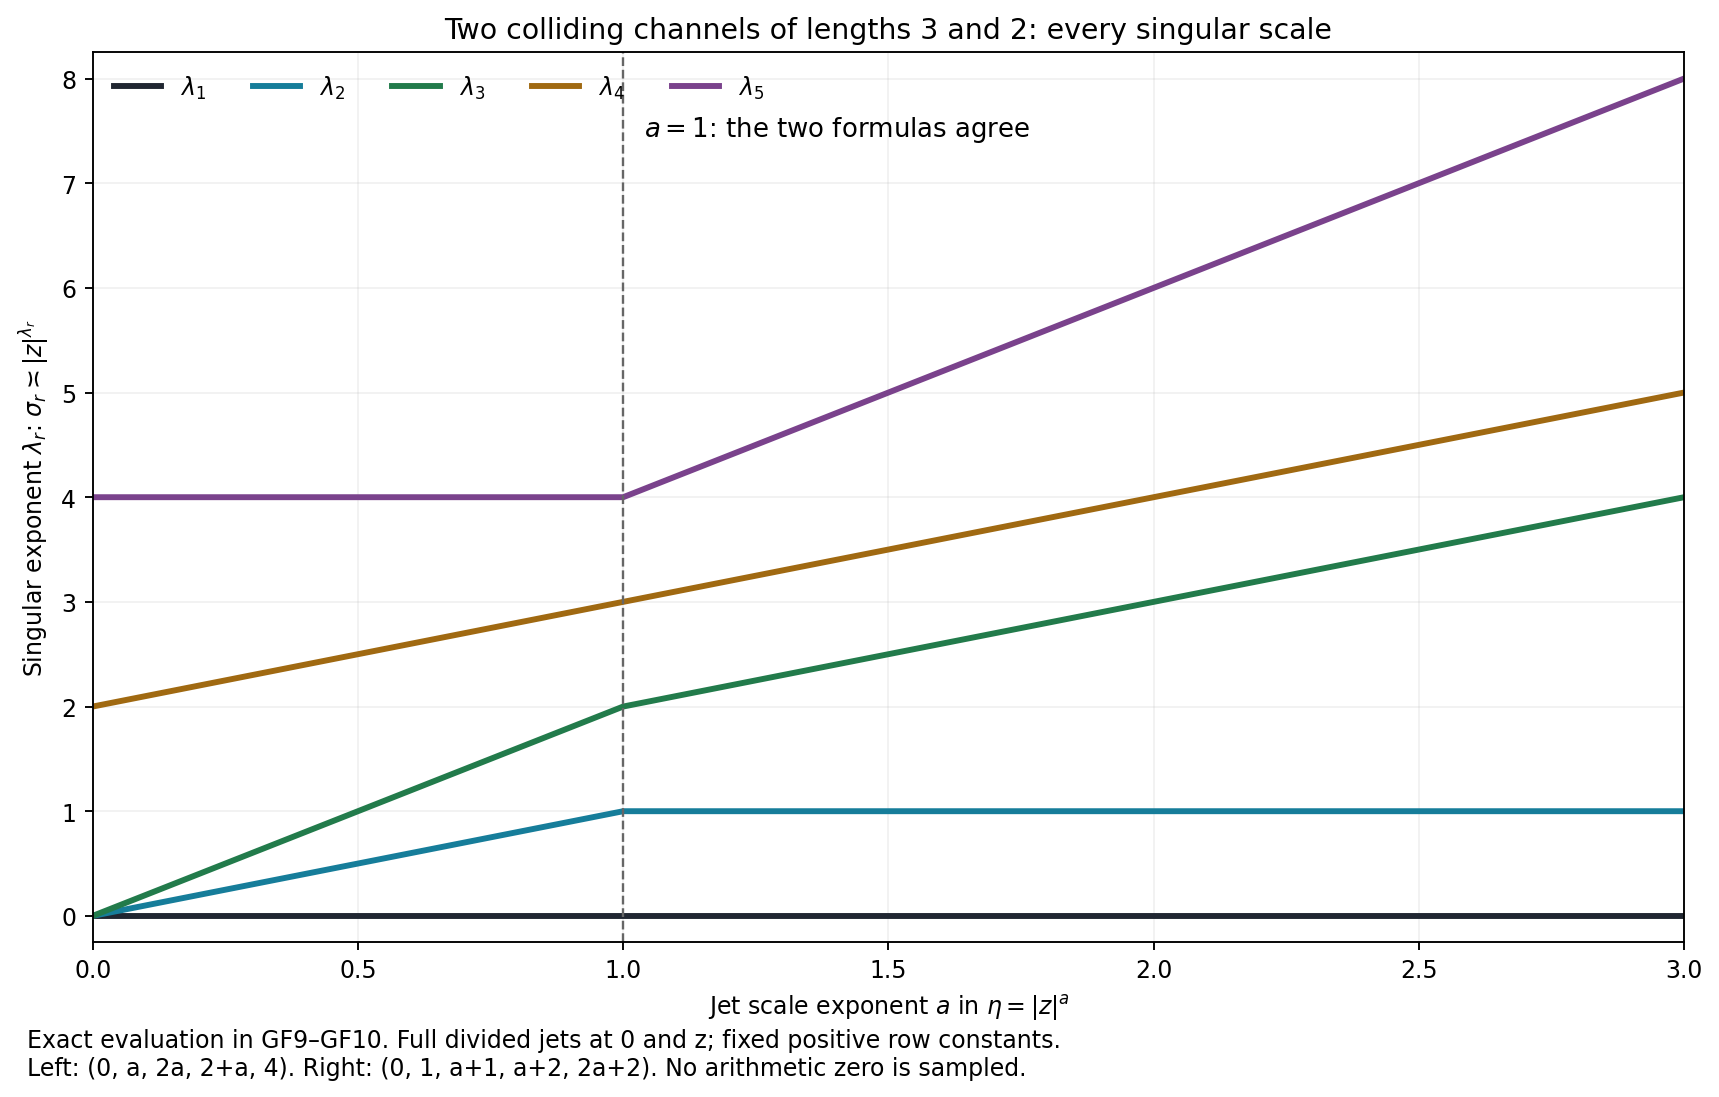
\includegraphics[width=\linewidth]{COLLISION_SCALE_EXACT.png}
\caption{The exact exponent list for channel lengths $e=3$, $f=2$.
The input is the full divided-jet map (GF8) with $\eta=|z|^a$.
Every line is the proved piecewise-linear expression (GF9)--(GF10),
not fitted singular-value data. The only transition is $a=1$.
The source of the plotted formulas is the complete proof above;
the reproducible figure script accompanies this note.}
\end{figure}
For any exterior inverse rank $r$, its divergence exponent is the sum
of the largest $\min(r,e+f)$ entries of (GF9) or (GF10). In particular
at $a=0$ this is $p(e+f-p)$, $p=\min(r,f)$, exactly as in input C10.
These statements concern the original two-channel evaluation and its
retained metric; additional unbounded coordinate factors must be kept
in that evaluation before these exponents are applied.

At $z=0$, the flat observation kernel is
$(u^e)/(u^{e+f})$, and the exact module map $u^ea\mapsto a\bmod u^f$
identifies it with $E_f=\C[u]/u^f$. The two-channel sequence is
\[
0\longrightarrow E_e\xrightarrow{p\mapsto(p,p\bmod u^f)}
E_e\oplus E_f\xrightarrow{(p,q)\mapsto q-p\bmod u^f}E_f
\longrightarrow0.
\tag{GF15}
\]
For $e>f$, (GF4)--(GF6) show leakage rank $f$ and reducing enlargement
equal to the whole two-channel space. For $e=f$, the diagonal is already
reducing and has zero leakage, while the flat kernel still has dimension
$e$. The module maps in (GF15), including the independent difference
channel, remain valid. At level $j<f$, weights $a_j,b_j>0$ give minimum
representative $(-b_jz/(a_j+b_j),a_jz/(a_j+b_j))$ and quotient norm
$a_jb_j|z|^2/(a_j+b_j)$, by completing the square. This positive quotient
norm is not a replacement for the vanishing flat observation norm.

\section{The actual source section and its complete additional minimum}
Let $\mathcal A_hP=P(-x\partial_x)F_h$ use the admitted divisor and
original source measure from input S1. At degree $2d-1$, let $H>0$ be
the complete Gram and $J$ the remainder map to $E_h$.
Then
\[
G_0=(JH^{-1}J^*)^{-1},\quad R_0=H^{-1}J^*G_0.
\]
The $d$ relation columns $B=(h,sh,\ldots,s^{d-1}h)$ span the full
kernel. With $W=B(B^*HB)^{-1/2}$, one has $JW=0$,
$W^*HW=I$ and $R_0^*HW=0$.
For the complete one-factor target jet metric $T_\eta$, put
\[
\Lambda_h=1+\|T_1^{-1/2}G_0T_1^{-1/2}\|,\quad
\tau_\eta=\Lambda_h\eta^{-2d_*},\quad
R_\eta=R_0+W(\tau_\eta T_\eta-G_0)^{1/2}.
\tag{GF16}
\]
Since $T_\eta\succeq\eta^{2d_*}T_1$ and
$G_0\preceq(\Lambda_h-1)T_1$, its positive square root exists and
\[
JR_\eta=I,\qquad R_\eta^*HR_\eta=\tau_\eta T_\eta.
\tag{GF17}
\]
The changed section, rather than a rescaled source mass, produces the
factor $\tau_\eta$. Tensoring these sections with $\beta$ gives degree
at most $\sum_i(2d_i-1)$ and metric
$(\prod_i\tau_{i,\eta})G_{\mathrm{cyc}}$.
Its class is the original $(\bigotimes_i U_i)\beta$ because the
difference from the literal sum polynomial belongs to the complete ideal
$(h_1(s_1),\ldots,h_k(s_k))$.

Hereafter $E$ denotes that original cyclic quotient. In the common
physical tensor Hilbert space, let $B_X:\C^{N+1}\to\mathscr H$ be the
original scalar-in-the-sum source and $R:E\to\mathscr H$ the constructed
tensor section. Their actual values are $J_N$ and $I_E$, respectively.
The equality of those values on equal physical representatives follows
from the common original quotient map, including the units above.
Set
\[
H_X=B_X^*B_X,\quad G=(J_NH_X^{-1}J_N^*)^{-1},\quad C=B_X^*R,
\]
\[
Z=R-B_XH_X^{-1}C,\quad H_Z=Z^*Z=R^*R-C^*H_X^{-1}C,
\quad F=I-J_NH_X^{-1}C.
\tag{GF18}
\]
Every mixed entry of $C$ is retained. Specifically, in original
coefficients it is the coefficient of $t^n$, multiplied by $n!$, in
\[
\sum_\alpha\beta_{\alpha,v}\prod_i
\left(\sum_{j=0}^N\frac{t^j}{j!}
\langle s^j,R_i e_{\alpha_i}\rangle_{w_{h_i}}\right).
\tag{GF19}
\]
The coefficients of the multinomial expansion are real, so (GF19)
retains the conjugate-linear first argument and every physical phase.

\begin{proposition}[Full source minimum]
The complete attained metric on $X_N+\im R$ is
\[
G_+=(G^{-1}+F H_Z^+F^*)^{-1}.
\tag{GF20}
\]
\end{proposition}
\begin{proof}
If $Za=0$, then $Ra=B_XH_X^{-1}Ca$ are equal physical source
representatives; applying their common quotient value gives $Fa=0$.
Hence $\ker H_Z\subset\ker F$. Let $U_+$ be a Euclidean orthonormal
frame of the positive eigenspace of $H_Z$, and write its positive
matrix there as $D_+$. Then $Z U_+D_+^{-1/2}$ is an orthonormal frame
of the actual normal source $\im Z$, and its value matrix is
$V_0=F U_+D_+^{-1/2}$. The orthogonal source sum has value covariance
$G^{-1}+V_0V_0^*$. Minimizing the full positive norm on every value
fibre gives its inverse, proving (GF20). Since
$V_0V_0^*=F H_Z^+F^*$, the formula is independent of the auxiliary
frame and is valid also when $H_Z$ is singular. No null source direction
has been inverted.
\end{proof}

For subsequent formulas write $V=F(H_Z^+)^{1/2}$; unused zero columns
are allowed. Thus $VV^*=F H_Z^+F^*$, with its exact physical meaning
fixed by the proof. The elementary identity, verified by multiplication,
is
\[
G_+=G-GV(I+V^*GV)^{-1}V^*G.
\tag{GF21}
\]

\section{New receivers for the original observation, kernel and signed current}
Let $\Lambda:E\twoheadrightarrow B$ be the original observation,
including its actual period and units, and let $I_K$ be any fixed
full-rank coordinate frame of $\ker\Lambda$. Define
\[
H=(\Lambda G^{-1}\Lambda^*)^{-1},\quad
\Omega=\Lambda^*H\Lambda,\quad
L=G^{-1}\Lambda^*H,\quad P=L\Lambda.
\tag{GF22}
\]
Here $L$ is the attained section, $P$ the projection to the observed
section, and $I-P$ the projection to the full original kernel. Put
$B_G=I+V^*GV$ and $B_\Omega=I+V^*\Omega V$.

\begin{theorem}[Exact observation and section changes]
For the complete enlarged source of (GF20),
\[
H_+=(H^{-1}+\Lambda VV^*\Lambda^*)^{-1},\qquad
\Omega_+=\Omega-\Omega V B_\Omega^{-1}V^*\Omega,
\tag{GF23}
\]
\[
L_+=L+(I-P)V B_\Omega^{-1}V^*\Lambda^*H,
\quad
P_+=P+(I-P)V B_\Omega^{-1}V^*\Omega.
\tag{GF24}
\]
Thus the change in the minimum lift lies in the actual original kernel.
For any original action $A:E\to E$, its observed action changes by
\[
\Lambda A L_+-\Lambda A L
=\Lambda A(I-P)V B_\Omega^{-1}V^*\Lambda^*H.
\tag{GF25}
\]
\end{theorem}
\begin{proof}
Push $G_+^{-1}=G^{-1}+VV^*$ through the unchanged onto map $\Lambda$;
this proves the first formula. Apply (GF21) to $H$ and $\Lambda V$
and multiply on both sides by $\Lambda^*,\Lambda$ to obtain the
second. For the section, multiply
$(G^{-1}+VV^*)\Lambda^*H_+$ and use
$I-V^*\Omega V B_\Omega^{-1}=B_\Omega^{-1}$.
The result is (GF24). Since $\Lambda(I-P)=0$, it is an exact difference
of sections into the original kernel. Applying $\Lambda A$ gives
(GF25); no invariance of that kernel under $A$ has been assumed.
\end{proof}

\begin{theorem}[Complete determinant allocation]
Set $K=I_K^*GI_K$ and $K_+=I_K^*G_+I_K$. Then
\[
\log\frac{\det G}{\det G_+}=\log\det B_G,
\quad
\log\frac{\det H}{\det H_+}=\log\det B_\Omega,
\tag{GF26}
\]
\[
\boxed{\log\frac{\det K}{\det K_+}
=\log\det B_G-\log\det B_\Omega.}
\tag{GF27}
\]
All three losses are nonnegative. Their sum relation is exact with
the fixed original coordinate frames. At every four-endpoint signed
return, apply those original signs to these same determinants.
\end{theorem}
\begin{proof}
The first two equalities follow by taking determinants of the covariance
updates. From (GF21), the determinant of $K_+$ relative to $K$ is
\[
\frac{\det\{B_G-V^*GI_KK^{-1}I_K^*GV\}}{\det B_G}.
\]
The exact projection identity
$G-GI_KK^{-1}I_K^*G=\Omega$ proves (GF27).
The comparison $0\preceq\Omega\preceq G$ implies
$I\preceq B_\Omega\preceq B_G$, giving nonnegativity.
These are matrix determinant identities on the full original kernel,
not rank-based allocations.
\end{proof}

The same proof works for any fixed inclusion $I_X$, with
$\Omega_X=G-GI_X(I_X^*GI_X)^{-1}I_X^*G$ in place of $\Omega$.
Therefore every original restriction receives the full comparison,
including those used for complementary returns.

For the retained native boundary columns $u_1,u_2$ and class $v$, put
\[
b_i=u_i^*\Omega v,\qquad
d_i=u_i^*\Omega V B_\Omega^{-1}V^*\Omega v.
\tag{GF28}
\]
Then $b_{i,+}=b_i-d_i$ exactly. With the fixed original denominator
$\omega>0$, the complete signed pairing obeys
\[
\boxed{\frac2\omega\Re(\overline{b_{1,+}}b_{2,+})
-\frac2\omega\Re(\overline b_1b_2)
=\frac2\omega\Re(-\overline b_1d_2-\overline d_1b_2
+\overline d_1d_2).}
\tag{GF29}
\]
This includes the correlated quadratic correction. It does not assign
the two complex corrections independent signs.
For $U=(u_1,u_2,v)$ the full loss matrix is
\[
U^*(\Omega-\Omega_+)U
=(B_\Omega^{-1/2}V^*\Omega U)^*
(B_\Omega^{-1/2}V^*\Omega U)\succeq0.
\tag{GF30}
\]
Its two-by-two minors and full determinant constrain the two $d_i$
and their shared diagonal losses simultaneously. If a different
denominator $\omega_+$ is introduced, the right side of (GF29) uses
$\omega_+$, and the additional exact term is
$(\omega/\omega_+-1)\,2\Re(\overline b_1b_2)/\omega$.
Thus (GF29) does not silently retain a denominator which has changed.

One useful exact differential version keeps the whole same added source
covariance. For $0\le t\le1$, put
$G_t=(G^{-1}+tVV^*)^{-1}$,
$H_t=(H^{-1}+t\Lambda VV^*\Lambda^*)^{-1}$ and
$\Omega_t=\Lambda^*H_t\Lambda$. Differentiation gives
\[
G_t'=-G_tVV^*G_t,\qquad
\Omega_t'=-\Omega_tVV^*\Omega_t,
\tag{GF31}
\]
\[
P_t'=(I-P_t)VV^*\Omega_t,\qquad
(\Lambda A L_t)'=\Lambda A(I-P_t)VV^*\Lambda^*H_t.
\tag{GF32}
\]
These follow by the product rule and the inverse derivative, so all
metric-induced motion of the section is present. They are a comparison
path between specified source minima; no new arithmetic zero family
is asserted.

\section{Acceptance and remaining native evaluations}
The assigned tensor-length formulas, reducing enlargement, fixed-scale
collision exponents, and full source minimum in the input check out.
Equations (GF9)--(GF14) evaluate the simultaneous collision algorithm
for every two-channel multiplicity pair and every $a\ge0$.
Equations (GF23)--(GF32) carry the entire added-source covariance
through the actual observation, full kernel, all fixed restrictions,
and signed boundary pairings. They supply the receiving maps needed
before a comparison to the original native determinants is made.

They do not evaluate $C$ in (GF18) on an unspecified arithmetic packet,
nor do they identify $G_+$ with the original $G$ or the constructed
section metric. For example $\log\det K$ is exactly
$\log\det K_++\log\det B_G-\log\det B_\Omega$; all three terms
are required for an absolute original allocation. The common positive
trace tolerance in the constructed metric does not remove these
determinants or the complex entries in (GF28).
The finite $\mathfrak{sl}_2$ commutators, Casimir and Vandermonde
identities used above are classical algebra; no novelty is claimed
for those identities. Their complete coordinate proofs retain the
actual metric and furnish the specified programme maps.
No statement of RH, its failure, or a Hodge-theoretic realization is
made here. All accepted identities in this note have the complete
finite proofs above. The companion checker exercises them in exact
coefficient examples; it is not a numerical evaluation of unknown
zeta roots, source moments or periods.


\clearpage
\section*{Evaluated tensor-to-sum projection and original metric comparison}

This calculation evaluates the reference cross Gram required in the
general-family receiving formula GF18--27. It retains the original
polynomial section and the original sum coordinate. The Gamma reference
and the arithmetic source are connected by a complete finite Gram
comparison at the end; they are not identified.

\section{Masses, coordinates and classical polynomial input}
For $a>0$, $b>0$ and a specified mass $\mu>0$, use
\begin{equation}\tag{MT1}
 d\sigma_{a,b,\mu}(y)=
 \mu\frac{2^{2a}}{2\pi b\Gamma(2a)}
 |\Gamma(a+iy/b)|^2\dd y.
\end{equation}
Here $b$ is a fixed coordinate scale, not a change in the arithmetic
roots. In the original physical variables $S_i=1/2+iy_i$, the source
sum is always $S=k/2+i\sum y_i$. The choice $a=1/4,b=2$ gives the
order-one Gamma convention with monic norm ratio $n(n-1/2)$, after
retaining the explicit mass in MT1.

Euler's beta formula \cite{MTBeta} and the change
$t=e^u/(1+e^u)$ give
\[
 \frac{|\Gamma(a+ix)|^2}{\Gamma(2a)}
 =\int_{\R}e^{ixu}(2\cosh(u/2))^{-2a}\dd u.
\]
The function on the right before Fourier transformation and each of
its derivatives are integrable. Integration by parts twice gives an
integrable Fourier transform, so Fourier inversion is valid. Evaluating
it at $u=bt$ proves
\begin{equation}\tag{MT2}
 \int e^{ity}\,d\sigma_{a,b,\mu}(y)
 =\mu\cosh(bt/2)^{-2a}.
\end{equation}
In particular MT1 has exactly the stated mass. To justify the
power-series operations below directly, fix $0<\theta<\pi$.
The function $(2\cosh(u/2))^{-2a}$ has an analytic branch on
$|\Im u|<\pi$, chosen positive on the real axis. On each closed
smaller strip its modulus is bounded by a constant times
$e^{-a|\Re u|}$. Shift the integration line to
$\Im u=\theta\operatorname{sgn}x$; the vertical sides tend to zero
by this bound. The Fourier integral is therefore bounded by
$C_{a,\theta}e^{-\theta|x|}$. MT1 consequently has every exponential
moment of order less than $\pi/b$. Dominated differentiation and
analytic continuation now justify the generating functions below
for sufficiently small complex parameters.

The monic Meixner--Pollaczek polynomials at angle $\pi/2$ have generating
function, in the DLMF convention \cite{MTMP},
\begin{equation}\tag{MT3}
 \sum_{n\ge0}\frac{p_n^{a,b}(y)}{n!}t^n
 =(1+b^2t^2/4)^{-a}
  \exp\left(\frac{2y}{b}\arctan(bt/2)\right).
\end{equation}
This is the original author generating function with argument $y/b$
and generating variable $bt/2$. The leading coefficient is one,
so the physical coordinate has not been removed. Apply MT2 with its
analytic continuation to the product of two generating functions.
Using $\cos(\arctan x+\arctan z)=(1-xz)/\sqrt{(1+x^2)(1+z^2)}$
gives $\mu(1-b^2ts/4)^{-2a}$. Comparing coefficients proves
\begin{equation}\tag{MT4}
 \langle p_n^{a,b},p_m^{a,b}\rangle_{\sigma_{a,b,\mu}}
 =\delta_{nm}\mu(b^2/4)^n n!(2a)_n.
\end{equation}
Thus the convolution of factors with the same $b$, parameters $a_i$
and masses $\mu_i$ is $\sigma_{A,b,\mu}$, where
$A=\sum_i a_i$, $\mu=\prod_i\mu_i$, by MT2 and uniqueness of the
Fourier transform. No factor mass has been set to one in these norms.

\section{An exact projection at every cutoff}
For a multi-index $\mathbf j$, put $n=\sum_i j_i$ and
$P_{\mathbf j}(\mathbf y)=\prod_i p_{j_i}^{a_i,b}(y_i)$.
For every scalar cutoff $N\ge n$, orthogonal projection in the complete
product Gamma measure onto polynomials of degree at most $N$ in
$Y=\sum_i y_i$ is
\begin{equation}\tag{MT5}\boxed{
 \Pi_N P_{\mathbf j}
 =\frac{\prod_i(2a_i)_{j_i}}{(2A)_n}\,p_n^{A,b}(Y).}
\end{equation}
For $N<n$ the projection is zero. Indeed multiplying the generating
functions MT3 proves the exact addition formula
\[
 p_m^{A,b}(Y)=\sum_{|\mathbf l|=m}
 \frac{m!}{\prod_i l_i!}\prod_i p_{l_i}^{a_i,b}(y_i).
\]
By MT4 its scalar product with $P_{\mathbf j}$ is zero unless $m=n$.
At $m=n$ it equals
$\mu(b^2/4)^n n!\prod_i(2a_i)_{j_i}$; divide by the full sum norm
$\mu(b^2/4)^n n!(2A)_n$ to obtain MT5. This proof covers every higher
scalar basis vector as well, so no further polynomial component
appears when the cutoff grows.

Retain the actual tensor polynomial section $R:E_k\to\C[\mathbf y]$
constructed from the original coefficients in GF16--17. Write it,
without altering any coefficients or units, as
\begin{equation}\tag{MT6}
 Rv=\sum_{|\mathbf j|\le D}c_{\mathbf j}(v)P_{\mathbf j},\qquad
 c_n(v)=\sum_{|\mathbf j|=n}
       c_{\mathbf j}(v)\frac{\prod_i(2a_i)_{j_i}}{(2A)_n}.
\end{equation}
Each $c_{\mathbf j}$ is a row on the original cyclic coefficient
space. Monic triangular division computes these rows from the original
section, including all complex phases. For the fixed one-factor degree
$d$ construction, $D\le k(2d-1)$.
By MT5, for every $N\ge D$,
\begin{equation}\tag{MT7}\boxed{\begin{gathered}
 \Pi_NR=\sum_{n=0}^D p_n^{A,b}(Y)c_n,\qquad
 H_Z^\Gamma=R^*H_\Gamma R-
 \sum_{n=0}^D\mu(b^2/4)^n n!(2A)_n c_n^*c_n,\\
 F_Z^\Gamma=I-\sum_{n=0}^D[p_n^{A,b}]c_n.
\end{gathered}}\end{equation}
Here $[p_n^{A,b}]$ is its actual class in $E_k$, evaluated at
$Y=(S-k/2)/i$ with the complete root polynomial and all jets.
The two matrices in MT7 are independent of $N$ once $N\ge D$.
Their Gram difference is positive semidefinite because it is the full
orthogonal normal component in the same product measure.

The exact complete reference minimum after adding this section to the
scalar source is therefore
\begin{equation}\tag{MT8}
 G^\Gamma_{+,N}=\left[(G^\Gamma_N)^{-1}+
 F_Z^\Gamma(H_Z^\Gamma)^+(F_Z^\Gamma)^*\right]^{-1},\quad N\ge\max(D,q-1).
\end{equation}
The finite proof is the orthogonal-source minimization GF18--21. The
kernel inclusion needed for its pseudoinverse holds here as well:
zero normal polynomial means equality with its scalar projection;
their original polynomial quotient values agree, so
$\ker H_Z^\Gamma\subset\ker F_Z^\Gamma$.
In particular the added covariance has an exact rank lower bound
\begin{equation}\tag{MT9}
 \rank\{F_Z^\Gamma(H_Z^\Gamma)^+(F_Z^\Gamma)^*\}
 =\rank F_Z^\Gamma\ge\max(0,q-D-1).
\end{equation}
To prove it, the kernel inclusion makes $F_Z^\Gamma$ vanish on the
zero eigenspace of $H_Z^\Gamma$, hence its multiplication by the
positive inverse square root has the same rank. The matrix subtracted
from the identity in MT7 factors through the $D+1$ scalar coefficients.
For any matrix $A$ of rank at most $D+1$, the equation
$v=(I-(I-A))v=Av$ on $\ker(I-A)$ shows that this kernel has dimension
at most $D+1$. This proves MT9. For the simple packet $q=(k+1)^2$ and
fixed $d$, it is a full order-$q$ source addition. It cannot be charged
as a bounded-rank change of the original observation.

\section{Exact comparison with the original arithmetic source}
All previous calculations use the reference metric, on the same
polynomial coefficient maps. The actual product measure is
$\prod_i w_{h_i}(y_i)\dd y_i$, and its scalar sum measure is the
original convolution. Set $L=\max(N,\max_i(2d_i-1))$ and form the
complete one-factor Grams $H_i^{\rm ar}(L)$ and $H_i^\Gamma(L)$ in
the original basis $1,y_i,\ldots,y_i^L$, with their actual masses.
They are positive definite. Define the finite original moment constants
\begin{equation}\tag{MT10}
 \ell_i=\lambda_{\min}((H_i^\Gamma)^{-1/2}H_i^{\rm ar}(H_i^\Gamma)^{-1/2}),
 \quad u_i=\lambda_{\max}((H_i^\Gamma)^{-1/2}H_i^{\rm ar}(H_i^\Gamma)^{-1/2}).
\end{equation}
These are explicit finite moment matrices; no numerical values are
assigned to an unspecified actual zero packet. Tensoring the positive
matrix inequalities and pulling back through the unchanged polynomial
map for the physical sum $X_N+\im R$ gives
\begin{equation}\tag{MT11}\boxed{
 (\prod_i\ell_i)G^\Gamma_{+,N}
 \preceq G^{\rm ar}_{+,N}\preceq
 (\prod_i u_i)G^\Gamma_{+,N}.}
\end{equation}
For completeness, if two positive source norms satisfy such inequalities,
their minima over each identical affine value fibre satisfy them by
taking the infimum of the lower and upper bounds. This proves MT11
and the same statement after any of the original restrictions or onto
observations. All scalar-source and tensor-source cross entries are
included before taking the infimum. For a rank-$r$ retained quotient
or restriction the logarithmic determinant difference is between
$r\sum_i\log\ell_i$ and $r\sum_i\log u_i$. The rank factor is retained.

\section{Every reference cutoff and its original restriction}
The scalar reference minimum in MT8 also has a fully evaluated matrix
in the same cyclic quotient. Put
\begin{equation}\tag{MT12}
 j_n=[p_n^{A,b}],\quad h_n=\mu(b^2/4)^n n!(2A)_n,\quad
 W=F_Z^\Gamma(H_Z^\Gamma)^+(F_Z^\Gamma)^*.
\end{equation}
Every entry of $j_n$ is computed by polynomial division by the complete
original root polynomial, or equivalently by its complete divided jets.
The recurrence
\[
 p_0=1,\quad p_1=y,\quad
 p_{n+1}=yp_n-(b^2/4)n(n+2A-1)p_{n-1}
\]
follows by differentiating MT3 and comparing coefficients. Thus it
computes $j_n$ without discarding repeated roots or using a root gap.
Since these monic polynomials are an orthogonal basis with squared
norms $h_n$, their original quotient covariance is their column sum.
Consequently, at every $N\ge\max(D,q-1)$,
\begin{equation}\tag{MT13}\boxed{
 G_N^+=\left(\sum_{n=0}^N\frac{j_nj_n^*}{h_n}+W\right)^{-1}.}
\end{equation}
Here $G_N^+$ denotes the complete reference metric $G^\Gamma_{+,N}$.
All dependence on the tensor section is the same matrix $W$ at every
such cutoff, with its complete rank from MT9.

Let $\Lambda:E_k\to B$ be any one of the original onto observations,
let $Z$ have columns forming a basis of its actual kernel, and set
$H_N=(\Lambda(G_N^+)^{-1}\Lambda^*)^{-1}$,
$K_N=Z^*G_N^+Z$. For $u=j_{N+1}/\sqrt{h_{N+1}}$, define the two
actual energies
\begin{equation}\tag{MT14}
 a_N=u^*G_N^+u,\qquad
 b_N=(\Lambda u)^*H_N(\Lambda u),\qquad 0\le b_N\le a_N.
\end{equation}
The complete adjacent returns are
\begin{equation}\tag{MT15}\boxed{\begin{gathered}
 \frac{\det G_{N+1}^+}{\det G_N^+}=\frac1{1+a_N},\qquad
 \frac{\det H_{N+1}}{\det H_N}=\frac1{1+b_N},\\
 \frac{\det K_{N+1}}{\det K_N}=\frac{1+b_N}{1+a_N}.
\end{gathered}}
\end{equation}
To prove this, MT13 gives the exact covariance increment $uu^*$.
Multiplication verifies
$G_{N+1}^+=G_N^+-G_N^+uu^*G_N^+/(1+a_N)$.
The rank-one determinant identity follows by choosing a basis whose
first vector is the rank-one column, or directly expanding the
determinant multilinearly; it proves the first two ratios in MT15.
For the kernel ratio it gives
$1-u^*G_N^+ZK_N^{-1}Z^*G_N^+u/(1+a_N)$.
The orthogonal projections for the metric $G_N^+$ satisfy
\[
 ZK_N^{-1}Z^*G_N^++(G_N^+)^{-1}\Lambda^*H_N\Lambda=I.
\]
Their ranges are the original kernel and its orthogonal complement:
the first is identity on that kernel and the second is its minimum
section projection. This proves the displayed identity and the
orthogonal decomposition $a_N=(a_N-b_N)+b_N$ into nonnegative
energies. Substitution proves the third ratio in MT15. Products of
these identities telescope over each of the original integration
windows; no separate allocation is assigned from a dimension alone.

MT7 evaluates the Gamma cross Gram and its normal-value matrix rather
than defining them through an unperformed projection. MT10--11 give
the exact original source map for this evaluation. MT12--15 evaluate
the full reference covariance and retain both actual observation
energies through each adjacent cutoff. They do not replace
the actual arithmetic cross Gram by the reference one or infer a
projected sign from a positive norm comparison. The outstanding native
calculation is now the correlated arithmetic comparison of these
specified matrices, with the same full kernel and all four endpoints.


\begin{figure}[p]\centering
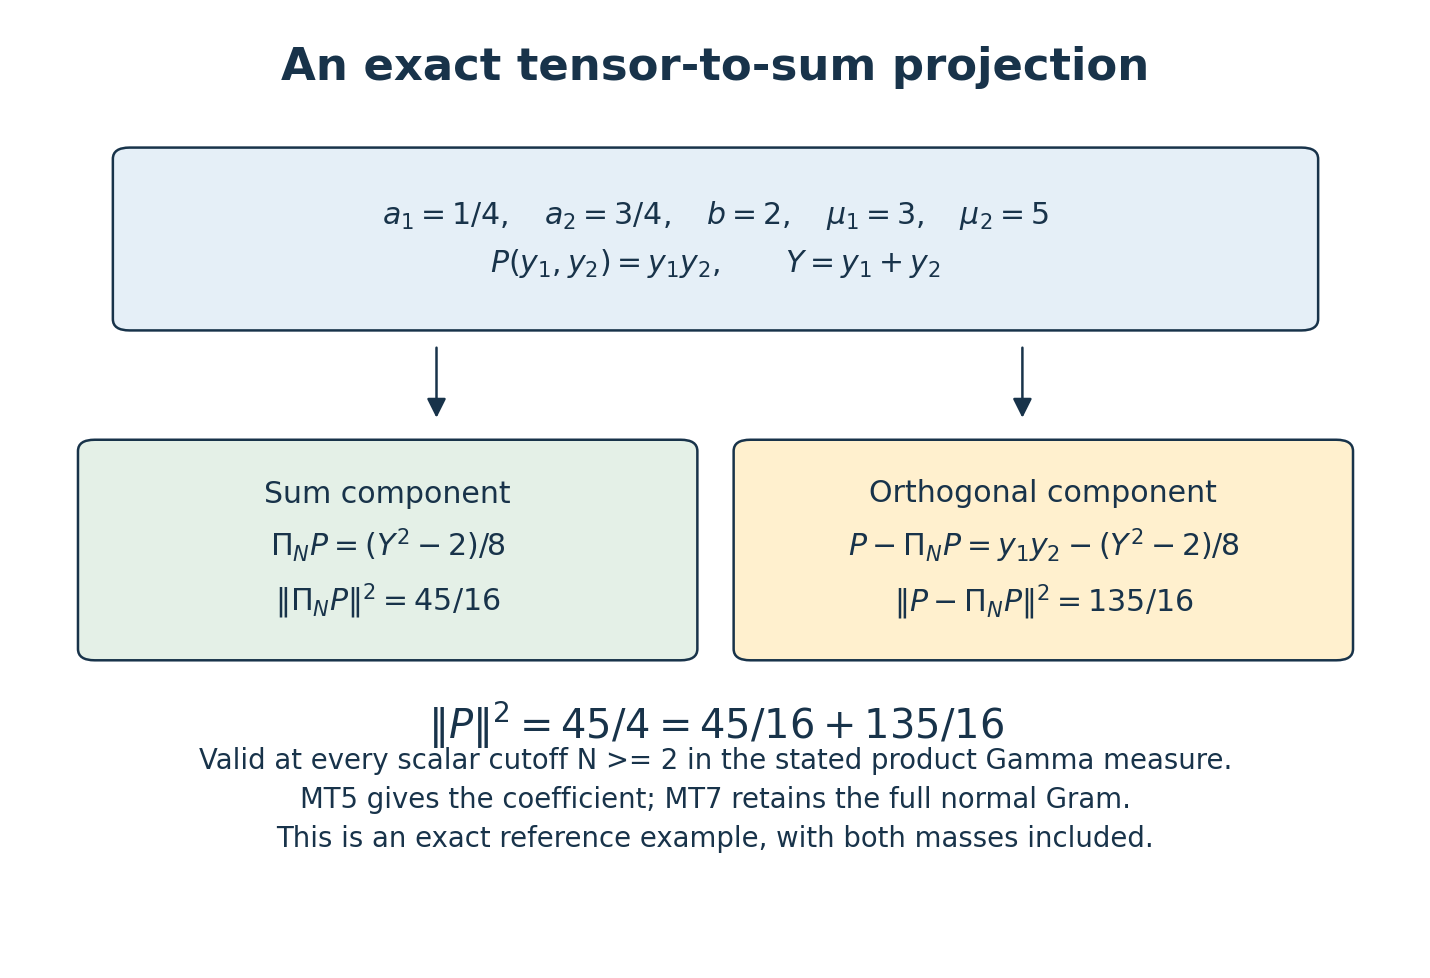
\includegraphics[width=\linewidth]{TENSOR_SUM_EXACT_PROJECTION.png}
\caption{A complete evaluation of MT5 with unequal Gamma parameters and both original masses. Every value is exact. Euler's beta integral and the Meixner--Pollaczek generating function are cited in MT1--4; the tensor projection and both norms are proved by MT4--5. MT10--11 connect this reference calculation to the unchanged arithmetic polynomial source.}
\end{figure}\clearpage

\clearpage
\section*{The complete arithmetic mixed-Gram return}

The reference projection MT5--7 is evaluated in closed coefficients
in the complete source construction of \cite{MAMT,MAGF}%
% BEGIN VERIFIED PUBLIC PROOF LINK
~\href{https://github.com/KokunoYumeto/zeta-function-research-reader/blob/main/workbenches/splitzero-tandem/continuations/20260921-kernel-degree-steps/providers/OBSERVATION_COMPLETE_PROOFS.tex\#L1629}{[proof MT1]} \href{https://github.com/KokunoYumeto/zeta-function-research-reader/blob/main/workbenches/splitzero-tandem/continuations/20260921-kernel-degree-steps/providers/OBSERVATION_COMPLETE_PROOFS.tex\#L1383}{[proof GF16]}%
% END VERIFIED PUBLIC PROOF LINK
{}.
Here the difference from the original arithmetic projection is carried
through its complete normal source, minimum, kernel and signed current.
There is no assumption that the metric difference is small or positive.

\section{The same polynomials and the two complete Grams}
Fix an original cutoff $N\ge\max(D,q-1)$. Use one finite coefficient
space containing the original scalar polynomials $X_N$ and the section
image $\im R$. It may be the complete tensor polynomial space of
individual degree at most $L$ from MT10. Its reference and arithmetic
Grams are $H_0>0,H_a>0$, with their actual masses. Put
\[
 \Delta=H_a-H_0,\quad B:\C^{N+1}\longrightarrow X_N,
 \quad A_0=B^*H_0B,\quad A=B^*H_aB.
 \tag{MA1}
\]
Here $B$ is the unchanged polynomial inclusion in the physical sum
$S=k/2+i\sum y_i$. On $X_N+\im R$ the original quotient value is
$\mathcal J$, so $\mathcal JB=J$ and $\mathcal JR=I_E$.
It is unnecessary to extend $\mathcal J$ to unrelated tensor classes.
Define the evaluated reference projection and normal component by
\[
 K_0=A_0^{-1}B^*H_0R,\quad Z_0=R-BK_0,\quad
 H_{Z,0}=Z_0^*H_0Z_0,\quad F_0=I-JK_0.
 \tag{MA2}
\]
MT5--7 give their actual coefficients; in particular $Z_0$ and $F_0$
are independent of the scalar cutoff once $N\ge D$, viewed as
polynomials and values. The new arithmetic data are precisely
\[
 E=B^*\Delta Z_0,\qquad D_0=Z_0^*\Delta Z_0.
 \tag{MA3}
\]
Every entry is a finite original moment integral. With monomial
exponents $\alpha,\beta$, the ambient matrices have entries
$\prod_i\int y_i^{\alpha_i+\beta_i}w_{h_i}(y_i)\,dy_i$
and the same products of the reference moments in MT2, respectively.
Conjugation of all polynomial coefficients is retained on the left.
Thus MA3 is a specified map from the original arithmetic moments,
including their complete divisors and phases, to the mixed correction.

\section{Exact projection and normal-Gram correction}
Let $K_a=A^{-1}B^*H_aR$ and $Z_a=R-BK_a$. Then
\begin{equation}\tag{MA4}\boxed{\begin{aligned}
 K_a&=K_0+A^{-1}E,& Z_a&=Z_0-BA^{-1}E,\\
 F_a&=F_0-JA^{-1}E,&
 H_{Z,a}&=H_{Z,0}+D_0-E^*A^{-1}E.
\end{aligned}}\end{equation}
Indeed $B^*H_0Z_0=0$ and $R=BK_0+Z_0$, hence
$B^*H_aR=AK_0+E$. This proves the first three formulas.
Expanding $(Z_0-BA^{-1}E)^*H_a(Z_0-BA^{-1}E)$ gives
$Z_0^*H_aZ_0-E^*A^{-1}E$, proving the last one. In particular the
two mixed terms do not disappear; they combine with the positive
square to give the displayed negative correction.

Both normal Grams have the same kernel,
\[
 \ker H_{Z,a}=\ker H_{Z,0}=\{v:Rv\in X_N\}
 \subset\ker F_a\cap\ker F_0.
 \tag{MA5}
\]
Positivity makes a zero Gram norm equivalent to the zero normal
polynomial. Both projections have exactly $X_N$ as their range, so
their normal polynomial vanishes exactly when $Rv\in X_N$.
Applying the same quotient value proves the kernel inclusion.
Consequently $Z_0v\mapsto Z_av$ is a well-defined bijection between
the two normal polynomial spaces; its inverse sends $Z_av$ back to
$Z_0v$. MA4 specifies this map in the original coefficients, with
both source norms retained.

Choose a matrix $U$ whose columns are any Euclidean basis of
$(\ker H_{Z,0})^\perp$. Write
$S_0=U^*H_{Z,0}U$, $S_a=U^*H_{Z,a}U$,
$V_0=F_0U$, and $T=JA^{-1}EU$. Both $S_0,S_a$ are positive
definite. The complete attained value covariances are
\begin{equation}\tag{MA6}\begin{aligned}
 C_0&=JA_0^{-1}J^*+V_0S_0^{-1}V_0^*,\\
 C_a&=JA^{-1}J^*+(V_0-T)S_a^{-1}(V_0-T)^*,\qquad
 G_0=C_0^{-1},\quad G_a=C_a^{-1}.
\end{aligned}\end{equation}
For a direct proof use the fixed independent source frame
$[B,Z_0U]$. Its reference Gram is $\operatorname{diag}(A_0,S_0)$,
its arithmetic Gram is
\[
 \begin{pmatrix}A&EU\\U^*E^*&S_0+U^*D_0U\end{pmatrix},
\]
and its unchanged quotient map is $[J,V_0]$.
Subtracting $BA^{-1}EU$ from the second block gives the arithmetic
orthogonal frame $[B,Z_aU]$ with Gram
$\operatorname{diag}(A,S_a)$ and value $[J,V_0-T]$.
For any positive source Gram $H$ and onto value matrix $Q$, the
minimum section is $H^{-1}Q^*(QH^{-1}Q^*)^{-1}$: substitution verifies
its value and its orthogonality to $\ker Q$. Its squared minimum
therefore has matrix $(QH^{-1}Q^*)^{-1}$. This proves MA6 without
inverting a null direction.

Put $\mathcal D=C_a-C_0$. Its full expansion is
\begin{equation}\tag{MA7}\boxed{\begin{aligned}
\mathcal D={}&J(A^{-1}-A_0^{-1})J^*
 +V_0(S_a^{-1}-S_0^{-1})V_0^*\\
 &-TS_a^{-1}V_0^*-V_0S_a^{-1}T^*
 +TS_a^{-1}T^*.
\end{aligned}}\end{equation}
All five terms follow by expansion of MA6. The first inverse difference
is $-A_0^{-1}(B^*\Delta B)A^{-1}$, and the second is
$-S_0^{-1}U^*(D_0-E^*A^{-1}E)US_a^{-1}$, as direct
multiplication verifies. These identities retain the correlations
between the arithmetic metric and the moving source projection.

\section{The original quotient, full kernel, action and phase}
Fix any original onto observation $\Lambda:E\to\mathcal B$.
For $i=0,a$ put
$Q_i=(\Lambda C_i\Lambda^*)^{-1}$,
$\Omega_i=\Lambda^*Q_i\Lambda$,
$L_i=C_i\Lambda^*Q_i$, and $P_0=L_0\Lambda$.
All maps use the original coefficient classes, period and physical
action $\mathcal A$. The inverse identity gives
\begin{equation}\tag{MA8}\boxed{\begin{aligned}
 Q_a-Q_0&=-Q_0\Lambda\mathcal D\Lambda^*Q_a,\\
 \Omega_a-\Omega_0&=-\Omega_0\mathcal D\Omega_a,\\
 L_a-L_0&=(I-P_0)\mathcal D\Lambda^*Q_a,\\
 \Lambda\mathcal A L_a-\Lambda\mathcal A L_0
 &=\Lambda\mathcal A(I-P_0)\mathcal D\Lambda^*Q_a.
\end{aligned}}\end{equation}
The third identity follows by inserting the first into
$C_a\Lambda^*Q_a-C_0\Lambda^*Q_0$; the fourth is its image under
the unchanged action. In particular the section difference takes
values in the original kernel since $\Lambda P_0=\Lambda$.
No invariance of that kernel under $\mathcal A$ is assumed.

For a fixed basis matrix $Z_K$ of this kernel let
$K_i=Z_K^*G_iZ_K$. Set
\[
 B_E=I+G_0^{1/2}\mathcal D G_0^{1/2},\qquad
 B_{\mathcal B}=I+Q_0^{1/2}\Lambda\mathcal D\Lambda^*Q_0^{1/2}.
\]
They are positive definite because they are congruent to $C_a$
and $\Lambda C_a\Lambda^*$, respectively. The exact three returns are
\begin{equation}\tag{MA9}\boxed{
 \frac{\det G_a}{\det G_0}=(\det B_E)^{-1},\qquad
 \frac{\det Q_a}{\det Q_0}=(\det B_{\mathcal B})^{-1},\qquad
 \frac{\det K_a}{\det K_0}=\frac{\det B_{\mathcal B}}{\det B_E}.}
\end{equation}
The first two are obtained by factoring $C_0^{1/2}$ or
$(\Lambda C_0\Lambda^*)^{1/2}$ in the covariance determinant.
For the third, choose any fixed right inverse $L$ of $\Lambda$.
The frame $[Z_K,L]$ is an isomorphism and block elimination in its
Gram gives
$|\det[Z_K,L]|^2\det G_i=\det K_i\det Q_i$.
This fixed factor cancels in the ratio, proving MA9. Logarithms of
MA9 may be summed with every original endpoint or window weight;
the same-class kernel term remains present in each sum.

Finally retain an original class $v$ and the original two boundary
vectors $u_1,u_2$ in these coordinates. The chosen vectors remain
fixed in the comparison; this includes the possibility that their
specified coefficients came from the arithmetic boundary calculation.
Define
\[
 b_j^i=u_j^*\Omega_i v,\qquad
 d_j=u_j^*\Omega_0\mathcal D\Omega_a v.
 \tag{MA10}
\]
Then $b_j^a=b_j^0-d_j$, and the complete phase correction is
\begin{equation}\tag{MA11}\boxed{
 \overline{b_1^a}b_2^a-\overline{b_1^0}b_2^0
 =-\overline{b_1^0}d_2-\overline{d_1}b_2^0+\overline{d_1}d_2.}
\end{equation}
Taking the particular real or imaginary part and original coefficient
in the native current preserves all three terms. Cauchy--Schwarz gives
the finite original-coordinate controls
\begin{equation}\tag{MA12}\begin{gathered}
 \|H_{Z,a}-H_{Z,0}\|\le\|D_0\|+\|A^{-1/2}E\|^2,\qquad
 \|F_a-F_0\|\le\|JA^{-1/2}\|\,\|A^{-1/2}E\|,\\
 |d_j|\le\|\Omega_0u_j\|\,\|\mathcal D\|\,\|\Omega_av\|.
\end{gathered}\end{equation}
Here all matrix norms are Euclidean spectral norms in the stated
original coefficient basis. These are exact finite bounds, with their
actual amplification factors still present. They assign no arithmetic
asymptotic coefficient or individual projected sign without evaluating
the original moments in MA3 and their correlations through MA7.

\section{Use in the current programme}
MT5--7 evaluate the reference projection, including every scalar
degree above the section degree. MA3--7 give the complete map from
the original arithmetic moment difference to its true normal source
and attained minimum. For higher scalar degrees the reference cross
coefficient vanishes exactly; the arithmetic coefficient is retained
in $B^*\Delta Z_0$. MA8--11 then carry this same correction through
the original quotient, its kernel and the actual phase. This is the
specific correlated arithmetic matrix that the next analytic estimate
must calculate. The finite identities here do not claim that estimate.



\clearpage
\begin{thebibliography}{99}

\bibitem{OHinput} User-supplied research continuation,
\emph{The original observation quotient retains the exponentially large
outgoing rank-one term}, received 20 September 2026, equations (4)--(45).
Exact original text and SHA256 retained in the private source ledger.
OH1--18 credit and prove its mathematical contribution.
\bibitem{BLinput} User-supplied research continuation,
\emph{Codex has now integrated substantial parts of the preceding work
into both repositories}, received 20 September 2026, Sections 2 and 4.
Exact original text and SHA256 retained in the private source ledger.
The occupation-space Section 5 is routed to the corresponding ES task.
\bibitem{SD} Split-Zero research programme, \emph{The original spectral
determinant and its small singular values}, SD1--28, result
SZ-20260920-053, 20 September 2026; full proof supplied with its edition.

% BEGIN VERIFIED PUBLIC PROOF LINK
\href{https://github.com/KokunoYumeto/zeta-function-research-reader/blob/5992ad50c0f2a06921f1fcaded7b4e38097c0739/workbenches/splitzero-tandem/continuations/20260920-original-kernel-mixed-determinants/providers/ORIGINAL_SPECTRAL_DETERMINANT.tex\#L34}{Source proof SD1}.
% END VERIFIED PUBLIC PROOF LINK
\bibitem{FW} Split-Zero research programme, \emph{Full-window source
products and the retained class}, FW1--7, FW40, FW44, FW46--52;
complete original conductor proof and LRS endpoint estimates cited
there with their full source identities. The exact provider is pinned
and retained with this result, including its bibliography.

% BEGIN VERIFIED PUBLIC PROOF LINK
\href{https://github.com/KokunoYumeto/zeta-function-research-reader/blob/5992ad50c0f2a06921f1fcaded7b4e38097c0739/workbenches/splitzero-tandem/continuations/20260920-original-kernel-mixed-determinants/providers/FULL_WINDOW_SOURCE_PRODUCTS.tex\#L28}{Source proof FW1}.
% END VERIFIED PUBLIC PROOF LINK
\bibitem{NG} Split-Zero research programme, \emph{Gaussian spectral
actions through the original arithmetic quotient}, NG1--27, and
\emph{The original equilibrium density, its second moment, and a signed
Gaussian return}, GM1--25, result SZ-20260920-052; published commit
\nolinkurl{98fd90e8eee771b09aa1167c87c0f36005a5b33b}.

% BEGIN VERIFIED PUBLIC PROOF LINK
\href{https://github.com/KokunoYumeto/zeta-function-research-reader/blob/5992ad50c0f2a06921f1fcaded7b4e38097c0739/workbenches/splitzero-tandem/continuations/20260920-original-kernel-mixed-determinants/providers/GAUSSIAN_EQUILIBRIUM_MOMENTS.tex\#L22}{Source proof GM1}. \href{https://github.com/KokunoYumeto/zeta-function-research-reader/blob/5992ad50c0f2a06921f1fcaded7b4e38097c0739/workbenches/splitzero-tandem/continuations/20260920-original-kernel-mixed-determinants/providers/GAUSSIAN_ARITHMETIC_RETURN.tex\#L31}{Source proof NG1}.
% END VERIFIED PUBLIC PROOF LINK
\bibitem{EM} Split-Zero research programme, \emph{Finite heat-trace
control under an original quotient-metric comparison}, EM1--30,
published commit \nolinkurl{b8113f664f0ee1964bfecbd6b07288c75b270857}.

% BEGIN VERIFIED PUBLIC PROOF LINK
\href{https://github.com/KokunoYumeto/zeta-function-research-reader/blob/5992ad50c0f2a06921f1fcaded7b4e38097c0739/workbenches/splitzero-tandem/continuations/20260920-original-kernel-mixed-determinants/providers/ENDPOINT_METRIC_HEAT.tex\#L38}{Source proof EM1}.
% END VERIFIED PUBLIC PROOF LINK
\bibitem{DLMF} T. H. Koornwinder, R. Wong, R. Koekoek,
R. F. Swarttouw and W. P. Reinhardt, \emph{Orthogonal Polynomials},
Chapter 18, NIST Digital Library of Mathematical Functions,
\url{https://dlmf.nist.gov/18.22.E8} and
\url{https://dlmf.nist.gov/18.23.E7}. The original recurrence and
generating equation enter the retained Gamma translation estimate;
author equation TeX and reading coverage were preserved with result052.
\bibitem{E1} N. M. Temme, \emph{Exponential, Logarithmic, Sine, and
Cosine Integrals}, Chapter 6, NIST Digital Library of Mathematical
Functions, equations 6.2.1, 6.2.3--4,
\url{https://dlmf.nist.gov/6.2.E1},
\url{https://dlmf.nist.gov/6.2.E3},
\url{https://dlmf.nist.gov/6.2.E4}, version 1.2.8, 15 September 2026.
The original author equation TeX was read in full and retained. BL5
uses the defining integral; its receiving identity is proved here.
\bibitem{Carlson} B. C. Carlson, \emph{Elliptic Integrals}, Chapter 19,
NIST Digital Library of Mathematical Functions, equations 19.2.4,
19.2.5 and 19.2.8(a,b), \url{https://dlmf.nist.gov/19.2}.
The original author equation TeX and reading coverage are retained
with the complete GM proof in result052. OH8 uses the same conventions.


\bibitem{CPProgramme} Split-Zero research programme, cumulative
\href{https://github.com/KokunoYumeto/zeta-function-research-reader/blob/5992ad50c0f2a06921f1fcaded7b4e38097c0739/workbenches/splitzero-tandem/continuations/20260920-original-kernel-mixed-determinants/cumulative/09_UPDATED_JOINT_NOTE.tex\#L1}{\texttt{09\_UPDATED\_JOINT\_NOTE.tex}}: OQC1--23 and OQX3 (literal
observation, conductor and orbit ranks); CAI16--25 (original source
comparison and multiplication); NCE1--21 and ORE1--23 (full-class
boundary, currents and original attained quotient). Exact file pins
and reading coverage accompany this derivation.

% BEGIN VERIFIED PUBLIC PROOF LINK
\href{https://github.com/KokunoYumeto/zeta-function-research-reader/blob/5992ad50c0f2a06921f1fcaded7b4e38097c0739/workbenches/splitzero-tandem/continuations/20260920-original-kernel-mixed-determinants/cumulative/09_UPDATED_JOINT_NOTE.tex\#L11282}{Source proof OQC1}.
% END VERIFIED PUBLIC PROOF LINK
\bibitem{CPOB} Split-Zero research programme,
\href{https://github.com/KokunoYumeto/zeta-function-research-reader/blob/487253b5b01851da5b9b98af4e146fecf1fab902/workbenches/splitzero-tandem/continuations/20260920-heat-literature-observed-class/HEAT_LITERATURE_AND_OBSERVED_CLASS.tex\#L1}{\texttt{HEAT\_LITERATURE\_AND\_OBSERVED\_CLASS.tex}}, OB1--20 and
OC50--74: original cardinal contraction, complete lower residual,
reverse lift, period coefficients, full unit phase and explicit corner
nonvanishing domain. The result is read in its original source coordinates.

% BEGIN VERIFIED PUBLIC PROOF LINK
\href{https://github.com/KokunoYumeto/zeta-function-research-reader/blob/487253b5b01851da5b9b98af4e146fecf1fab902/workbenches/splitzero-tandem/continuations/20260920-heat-literature-observed-class/HEAT_LITERATURE_AND_OBSERVED_CLASS.tex\#L1223}{Source proof OB1}.
% END VERIFIED PUBLIC PROOF LINK
\bibitem{CPDLMF18} T. H. Koornwinder, R. S. C. Wong, R. Koekoek and
R. F. Swarttouw, with W. P. Reinhardt, \emph{Orthogonal Polynomials},
NIST Digital Library of Mathematical Functions, Chapter 18,
equation 18.23.7, \url{https://dlmf.nist.gov/18.23.E7}.
The exact Meixner--Pollaczek generating function is the human source
for the unchanged Gamma translation estimate in (CP21)--(CP22).


\bibitem{GFVandermonde} R. Roy, F. W. J. Olver, R. A. Askey,
R. Wong and W. P. Reinhardt, \emph{Algebraic and Analytic Methods},
Chapter 1, NIST Digital Library of Mathematical Functions,
equation 1.3.13, \url{https://dlmf.nist.gov/1.3.E13},
version 1.2.8, 15 September 2026. The original author equation TeX
was read and retained. The falling-factorial determinant above is
obtained from that monomial determinant by a triangular basis change
with diagonal entries one, preserving its complete nonzero factor.


\bibitem{MTBeta} R. A. Askey and R. Roy, \emph{Gamma Function}, Chapter 5,
NIST Digital Library of Mathematical Functions, Euler beta integral,
equation 5.12.1, \url{https://dlmf.nist.gov/5.12.E1}.
The original author equation TeX was read and retained. Its use here
includes the explicit real-line change of variables and Fourier inversion.
\bibitem{MTMP} T. H. Koornwinder, R. Wong, R. Koekoek, R. F. Swarttouw
and W. P. Reinhardt, \emph{Orthogonal Polynomials}, Chapter 18,
NIST Digital Library of Mathematical Functions, Meixner--Pollaczek
generating function 18.23.7, \url{https://dlmf.nist.gov/18.23.E7}.
The original author equation TeX was read in full. MT3 states every
coordinate and monic factor in its application; MT4--5 prove the
orthogonality and tensor projection used here.


\bibitem{MAMT} Split-Zero research programme, \emph{An evaluated tensor-to-sum
projection and the full native source comparison}, MT1--15,
20 September 2026, supplied in full with this edition. MT1--5 cite
R. A. Askey and R. Roy's Euler beta integral and T. H. Koornwinder,
R. Wong, R. Koekoek, R. F. Swarttouw and W. P. Reinhardt's
Meixner--Pollaczek generating function, NIST DLMF5.12.1 and18.23.7;
original author equation TeX and exact uses are retained.

% BEGIN VERIFIED PUBLIC PROOF LINK
\href{https://github.com/KokunoYumeto/zeta-function-research-reader/blob/main/workbenches/splitzero-tandem/continuations/20260921-kernel-degree-steps/providers/OBSERVATION_COMPLETE_PROOFS.tex\#L1629}{Source proof MT1}.
% END VERIFIED PUBLIC PROOF LINK
\bibitem{MAGF} Split-Zero research programme, \emph{General tensor families:
complete collision scales and original observation receivers},
GF16--32,20 September2026, supplied in full. MA4--12 derive the
additional arithmetic comparison from the unchanged source maps.
The underlying positive matrix and inverse identities are classical;
their complete coordinate proofs are included here.


% BEGIN VERIFIED PUBLIC PROOF LINK
\href{https://github.com/KokunoYumeto/zeta-function-research-reader/blob/main/workbenches/splitzero-tandem/continuations/20260921-kernel-degree-steps/providers/OBSERVATION_COMPLETE_PROOFS.tex\#L1383}{Source proof GF16}.
% END VERIFIED PUBLIC PROOF LINK
\end{thebibliography}
\end{document}
